% documentclass options:
\documentclass[11pt,
  a4paper,
  parskip=half, % This is some extra vertical space between paragraphs, the suggestion is 2cm which is really ugly, so we use what koma script gives us
  % you can also set it to full for even more space. But there is a bad tex style decision: parskip also changes the spacing between listitems such as
  % enumerate and itemize. For this purpose we include the enumitem package and set itemsep=.5em, of course you can change this
  BCOR=10mm, % BCOR is binding correction
  % if you'd rather have a one sided thesis, add `oneside' to the documentclass
  % oneside,
  % ngerman is needed for hyphenation if the thesis contains parts written in German, switch order with english if you write mainly in English.
  % Remember to change order in the babel package (below) as well.
  % Last language is the preferred one.
  english]{scrbook}
\usepackage[english]{babel} % If you write mainly in English change order to ngerman, english. Also change that in the documentclass options above.
% Include of titling must happen before \title etc.
% that's why it's not in setup.tex
\usepackage{titling}
\title{Benchmark of RISC-V in BTOR2}
\author{Jan Krister Möller}

% Change to your first examiner
% The ~ enables non sentence spacing after a period
\newcommand{\firstexaminer}{Dr.~Mathias Fleury}
% Change to your second examiner, some undergraduate studies don't have a second examiner
% in this case just comment out the following line
% \newcommand{\secondexaminer}{Prof.~Dr.~Wile E. Coyote}
% Change to your adivers
% \newcommand{\advisers}{Terence Hill, Bud Spencer}

% include all packages and define commands in setup.tex

%------------------------------------------------------------------------------
%       package includes
%------------------------------------------------------------------------------
% font encoding is set up for pdflatex, for other environments see
% http://tex.stackexchange.com/questions/44694/fontenc-vs-inputenc
\usepackage[T1]{fontenc}  % 8-bit fonts, improves handling of hyphenations
% provides `old' commands for table of contents. Eases the ability to switch
% between book and scrbook
\usepackage{scrhack}


% ------------------- layout, default -------------------
% adjust the style of float's captions, separated from text to improve readabilty
\usepackage[labelfont=bf, labelsep=colon, format=hang, textfont=singlespacing]{caption}
% With format = hang your caption will look like this:
% Figure 1: Lorem ipsum dolor sit amet,
%           consectetuer adipiscing elit.
%           Ut purus elit, vestibulum
% If you instead want
% Figure 1: Lorem ipsum dolor sit amet,
% consectetuer adipiscing elit. Ut purus
% elit, vestibulum
% change to format=plain
\usepackage{chngcntr}  % continuous numbering of figures/tables over chapters
\counterwithout{equation}{chapter}
\counterwithout{figure}{chapter}
\counterwithout{table}{chapter}

% Uncomment the following line if you switch from scrbook to book
% and comment the setkomafont line
%\usepackage{titlesec}  % remove "Chapter" from the chapter title
%\titleformat{\chapter}[hang]{\bfseries\huge}{\thechapter}{2pc}{\huge}
\setkomafont{chapter}{\normalfont\bfseries\huge}

\usepackage{setspace}  % Line spacing
\onehalfspacing
% \doublespacing  % uncomment for double spacing, e.g. for annotations in correction

% ------------------- functional, default-------------------
\usepackage[dvipsnames]{xcolor}  % more colors
\usepackage{array}  % custom format per column in table - needed on the title page
\usepackage{graphicx}  % include graphics
\usepackage{subfig}  % divide figure, e.g. 1(a), 1(b)...
\usepackage{amsmath}  % |
\usepackage{amsthm}   % | math, bmatrix etc
\usepackage{amsfonts} % |
\usepackage{calc}  % calculate within LaTeX
\usepackage[unicode=true,bookmarks=true,bookmarksnumbered=true,
    bookmarksopen=true,bookmarksopenlevel=1,breaklinks=false,
    pdfborder={0 0 0},backref=false,colorlinks=false]{hyperref}
\usepackage{etoolbox} % if-else commands


%==========================================
% You might not need the following packages, I only included them as they
% are needed for the example floats
% ------------------- functional, custom -------------------
\usepackage[boxed]{algorithm2e}
\usepackage{bm}  % bold greek variables (boldmath)
\usepackage{tikz}
\usetikzlibrary{positioning}  % use: above left of, etc

% Required for the ToDo list.
\usepackage{ifthen}

% Improves general appearance of the text
\usepackage[protrusion=true,expansion=true, kerning]{microtype}
\usepackage{enumitem}
% Nicer font for pdf rendering.
%\usepackage{lmodern}

% For nicer looking tables.
\usepackage{booktabs}

% You don't need this, just for demonstration of a longer caption.
\usepackage{lipsum}

%------------------------------------------------------------------------------
%       (re)new commands / settings
%------------------------------------------------------------------------------
% ----------------- referencing ----------------
\newcommand{\secref}[1]{Section~\ref{#1}}
\newcommand{\chapref}[1]{Chapter~\ref{#1}}
\renewcommand{\eqref}[1]{Equation~(\ref{#1})}
\newcommand{\figref}[1]{Figure~\ref{#1}}
\newcommand{\tabref}[1]{Table~\ref{#1}}
\newcommand{\algoref}[1]{Algorithmus~\ref{#1}}

% ------------------- colors -------------------
\definecolor{darkgreen}{rgb}{0.0, 0.5, 0.0}
% Colors of the Albert Ludwigs University as in
% https://www.zuv.uni-freiburg.de/service/cd/cd-manual/farbwelt
\definecolor{UniBlue}{RGB}{0, 74, 153}
\definecolor{UniRed}{RGB}{193, 0, 42}
\definecolor{UniGrey}{RGB}{154, 155, 156}


% ------------------- layout -------------------
% prevents floating objects from being placed ahead of their section
\let\mySection\section\renewcommand{\section}{\suppressfloats[t]\mySection}
\let\mySubSection\subsection\renewcommand{\subsection}{\suppressfloats[t]\mySubSection}



% ------------------- math formatting commands -------------------
% define vectors to be bold instead of using an arrow
\renewcommand{\vec}[1]{\mathbf{#1}}
\newcommand{\mat}[1]{\mathbf{#1}}
% tag equation with name
\newcommand{\eqname}[1]{\tag*{#1}}


% ------------------- pdf settings -------------------
% ADAPT THIS
\hypersetup{pdftitle={\thetitle},
    pdfauthor={\theauthor},
    pdfsubject={Undergraduate thesis at the Albert Ludwig University of Freiburg},
    pdfkeywords={deep learning, awesome algorithm,  undergraduate thesis},
    pdfpagelayout=OneColumn, pdfnewwindow=true, pdfstartview=XYZ, plainpages=false}


%==========================================
% You might not need the following commands, I only included them as they
% are needed for the example floats

% ------------------- Tikz styles -------------------
\tikzset{>=latex}  % arrow style


% ------------------- algorithm ---------------------
% Command to align comments in algorithm
\newcommand{\alignedComment}[1]{\Comment{\parbox[t]{.35\linewidth}{#1}}}
% define a foreach command in algorithms
\SetArgSty{textrm}
\SetAlgoInsideSkip{smallskip}
\IncMargin{5pt}
% line spacing should be 1.5
\renewcommand{\baselinestretch}{1.5}

% set distance between items in a list, for more details see the
% enumitem package: https://www.ctan.org/pkg/enumitem
\setlist{itemsep=.5em}

% use ra in your tables to increase the space between rows
% 1.3 should be fine
\newcommand{\ra}[1]{\renewcommand{\arraystretch}{#1}}

% ToDo counters
\usepackage{ifthen} %für whiledo-Schleife
\newcounter{todos}
\setcounter{todos}{0}
\newcounter{extends}
\setcounter{extends}{0}
\newcounter{drafts}
\setcounter{drafts}{0}

% ------------------- marker commands -------------------
% ToDo command
\newcommand{\todo}[1]{\textbf{\textcolor{red}{(TODO: #1)}}\refstepcounter{todos}\label{todo \thetodos}}
\newcommand{\extend}[1]{\textbf{\textcolor{darkgreen}{(EXTEND: #1)}}\refstepcounter{extends}\label{extend \theextends}}
% Lighter color to note down quick drafts
\newcommand{\draft}[1]{\textbf{\textcolor{NavyBlue}{(DRAFT: #1)}}\refstepcounter{drafts}\label{draft \thedrafts}}

% microtype with lmodern, see https://tex.stackexchange.com/questions/75305/microtype-warning-with-lmodern-package-and-koma-script
%\DeclareMicrotypeAlias{lmss}{cmr}


\begin{document}\pagestyle{empty} % no header and no page number
% disable hyper links to remove warning "destination with same identifier"
% this means within this section nothing can be referenced with a hyperlink
\hypersetup{pageanchor=false}

% enable/disable, depending on your chosen language

\begin{titlepage}
	\begin{center}

		\newcommand{\HorizontalLine}{\rule{\linewidth}{0.3mm}}

		{\Large Bachelor Thesis}\\[1.3cm]

		% _____________________________________________________________________________
		\HorizontalLine \\[0.4cm]
		% Write your title in a fancy way like this if you want to customize it, otherwise simply let tex do it for you
		% \begin{spacing}{3}
		%     {\huge \bfseries The Long, Long } \\
		%     {\huge \bfseries Long Long} \\
		%     {\huge \bfseries Title}\\
		% \end{spacing}
		{ \huge \bfseries \thetitle }
		\HorizontalLine \\[1.5cm]
		% _____________________________________________________________________________

		{\Huge \theauthor} \\[2cm]

		\begin{tabular}[hc]{>{\huge}l >{\huge}l}
			Examiner: & \firstexaminer \\[0.3cm]
			%  Advisers: & \advisers \\[1.2cm]
		\end{tabular}
		\vfill  % move the following text to the bottom

		\Large {
			University of Freiburg\\
			Faculty of Engineering\\
			Department of Computer Science\\
			Chair of Computer Architecture\\[1cm]

			\today
		}
	\end{center}
\end{titlepage}

\thispagestyle{empty}
% title page back
\ \vfill \ \\  % at least one space required before vfill
\
\textbf{Writing Period}            \smallskip{} \\
24.\,06.\,2025 -- 24.\,09.\,2025   \bigskip{} \\
\
\textbf{Examiner}                  \smallskip{} \\
\firstexaminer                     \bigskip{} \\
\
% If there is a second examiner include it
\ifdef{\secondexaminer}
{
	% Include
	\textbf{Second Examiner}       \smallskip{} \\
	\secondexaminer                \bigskip{} \\
	\
}
{
	% No second examiner, ignore
}
%\textbf{Advisers}                  \smallskip{} \\
%\advisers

%\input{chapters/0_0-titlepage_de}

\pagestyle{plain} % remove chapter name from top, page number at the bottom
% use \pagestyle{headings} for having the chapter on top of the pages
% if you wang a more fancy header use \usepackage[automark,headsepline]{scrlayer-scrpage}
% and read about it in the KOMA script documentation, https://www.ctan.org/pkg/koma-script
\frontmatter % roman page numbers

% Copied from the official declaration from the examination office (typos fixed).
% Please double check the wording on their website and report changes.
% (https://www.tf.uni-freiburg.de/de/studium-lehre/a-bis-z-studium/dokumente/Declarationforthefinalthesis.pdf)

\chapter*{Declaration}

I hereby declare that I am the sole author and composer of my thesis and that
no other sources or learning aids, other than those listed, have been used.
Furthermore, I declare that I have acknowledged the work of others by providing
detailed references of said work. \newline I hereby also declare that my Thesis
has not been prepared for another examination or assignment, either wholly or
excerpts thereof. \\[3\normalbaselineskip]
\begin{tabular}{p{\textwidth/2} l}
  \rule{\textwidth/3}{0.4pt} & \rule{\textwidth/3}{0.4pt} \\
  Place, Date                & Signature
\end{tabular}


\chapter*{Declaration on Usage of generative AI}

I hereby declare that, with the approval of my examiner, I have employed the
generative AI tool \dq GitHub Copilot\dq\ during the preparation of this thesis
solely for spellchecking and enhancing the formality of my written expression.
Furthermore, I expressly confirm that this tool was not used to generate data
or as a source of factual information or content for this thesis.\\[3\normalbaselineskip]
\begin{tabular}{p{\textwidth/2} l}
    \rule{\textwidth/3}{0.4pt} & \rule{\textwidth/3}{0.4pt} \\
    Place, Date                & Signature
\end{tabular}

\chapter*{Abstract}

RISC-V is an open-source instruction set architecture that is
increasingly adopted in both research and industry due to its
flexibility and extensibility \cite{riscv-isa, eu}. Formal
verification, particularly bounded model checking, is essential for
ensuring the correctness of such architectures in safety-critical
contexts \cite{BiereBMC}. BTOR2 has become a standard format for
word-level hardware model checking \cite{btor2, HWMCC}.

This thesis presents tools for translating RISC-V processor states
into BTOR2 models and reconstructing states from model checker
witnesses. The correctness of the models is validated by comparing
single-instruction execution against a reference RISC-V simulator
\cite{repoSim}. Benchmarking is performed to evaluate the feasibility
of this approach using the model checkers btormc, AVR, and Pono
\cite{btor2, avrPaper, ponoPaper}, with respect to instruction count,
address space, and memory initialization. The results show that model
checkers which perform best in general competitions do not
necessarily excel for my iteration-heavy RISC-V models..

\tableofcontents

\listoffigures

\listoftables

\listofalgorithms

\hypersetup{pageanchor=true} % re-enable hyperlinking

\mainmatter % Arabic page numbers

\chapter{Motivation}\label{chap:motivation}
This is a template for an undergraduate or master's thesis.
The first sections are concerned with the template itself. If this is your first
thesis, consider reading.

\chapter{RISC-V}\label{chap:riscv}

As the first foundation for my benchmarks and, consequently, this
thesis, I will discuss RISC-V and its operational principles.

\section{Overview}

RISC-V is an open-source instruction set architecture (ISA) first
published in May 2011 by A. Waterman et al. \cite{first_riscv}. As
indicated by its name, it is based on the RISC design philosophy.
RISC stands for Reduced Instruction Set Computer and its concept is
to only include a small set of elemental and easy to execute
instructions. With this, the decoding and execution of instructions
can be faster compared to CISC (Complex Instruction Set Computer)
design philosophy.

Since 2015, the development of RISC-V has been coordinated by the
RISC-V International Association, a non-profit corporation based in
Switzerland since 2020 \cite{riscvorg}. Its objectives include
providing an \emph{open} ISA that is freely available to all, a
\emph{real} ISA suitable for native hardware implementation, and an
ISA divided into a \emph{small} base integer ISA usable
independently, for example in educational contexts, with optional
standard extensions to support general-purpose software development
\cite[Chapter 1]{riscv-isa}.

Currently, RISC-V comprises four base ISAs: RV32I, RV64I, RV32E, and
RV64E, which can be extended with one or more of the 47 ratified
extension ISAs \cite[Preface]{riscv-isa}.

For the purposes of this work, I focus on a subset of the RV64I ISA.

\section{The RV64I ISA} \label{sec:riscvIsa}
RV64I is not overly complex, but its structure is essential for
understanding the subsequent work presented in this thesis.
Therefore, I will explain all elements relevant to my work.

RV64I features 32 64-bit registers, labeled $x0$–$x31$, where $x0$ is
hardwired to zero across all bits. Registers $x1$–$x31$ are
general-purpose and may be interpreted by various instructions as
collections of booleans, two's complement signed binary integers, or
unsigned integers. Additionally, there is a non-accessible register
called $pc$, which serves as the program counter and holds the
address of the current instruction \cite[Chapters 4.1,
      2.1]{riscv-isa}.

In RV64I, memory addresses are 64 bits in size. As the memory model
is defined to be single-byte addressable, the address space of RV64I
encompasses $2^{64}$ bytes \cite[Chapter 1.4]{riscv-isa}. The format
of the memory is little endian, so the lower bits of a number are
placed at lower addresses.

Like nearly all standard ISAs of RISC-V, RV64I employs a standard
instruction encoding length of 32 bits, or one \emph{word}. Only the
compressed extension named C introduces instructions with a length of
16 bits \cite[Chapter 1.5]{riscv-isa}, but this special case is not
considered here. All RV64I instructions are encoded in one of the six
formats illustrated in \figref{fig:rv64i_formats}. These formats may
consist of
\begin{itemize}
      \item The $opcode$:\\ The opcode is used to differentiate between groups of
            instructions. It also defines the format type of the instruction.
      \item $rd$:\\ This is the destination register.
      \item $funct3$:\\ This is used to differentiate between instructions with
            the same $opcode$.
      \item $rs1$ \& $rs2$:\\ These are the source registers.
      \item $funct7$:\\ This is used for further distinctions between
            instructions if there are more than eight instructions in an opcode
            group and $funct3$ does not suffice.
      \item $imm$:\\ This is an immediate value. In square brackets after $imm$
            is designated a subfield of the immediate which is represented by
            these bits. From these subfields, non-defined lower bits are filled
            with zeros whereas the highest defined bit is sign-extended to fill
            all non-defined higher bits.
\end{itemize}

\begin{figure}[t]
    \begin{centering}
        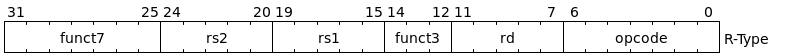
\includegraphics[width = \textwidth]{figures/2-RiscV/R.png}\\
        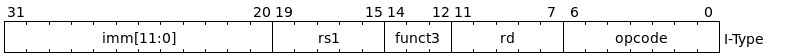
\includegraphics[width = \textwidth]{figures/2-RiscV/I.png}\\
        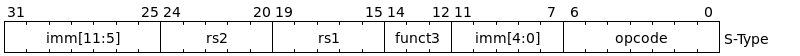
\includegraphics[width = \textwidth]{figures/2-RiscV/S.png}\\
        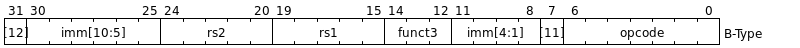
\includegraphics[width = \textwidth]{figures/2-RiscV/B.png}\\
        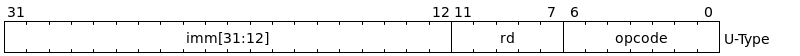
\includegraphics[width = \textwidth]{figures/2-RiscV/U.png}\\
        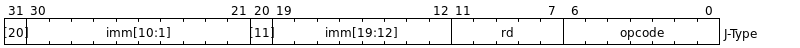
\includegraphics[width = \textwidth]{figures/2-RiscV/J.png}
        \caption[RV64I encoding formats]{RV64I encoding formats, used in \cite[Chapter 2.3]{riscv-isa}\todo{Kopie richtig angeben}}
        \label{fig:rv64i_formats}
    \end{centering}
\end{figure}


The design of these formats results in the following features:
\begin{itemize}
      \item Due to RISC-V's little-endian nature, the $opcode$, which encodes the
            general instruction, is always read first. Further specification of
            the instruction via $funct3$ and $funct7$ is consistently located at
            the same positions.
      \item If utilized by the instruction, $rd$, $rs1$, and $rs2$ are also
            always found in the same locations, simplifying decoding.
      \item The highest bit of $imm$ is always bit 31, making it straightforward
            to sign-extend the immediate value.
\end{itemize}

The instructions relevant to my work are listed in
\tabref{tab:rv64i-instructions} I have divided the instructions in
\tabref{tab:rv64i-instructions} into nine groups based on their
operations.

\texttt{LUI} and \texttt{AUIPC} move a high immediate into $rd$. In
the case of \texttt{AUIPC}, the $pc$ is added to this value.
\texttt{JAL} and \texttt{JALR} instructions are unconditional jumps,
where for \texttt{JAL} $imm$ is added to $pc$ and for \texttt{JALR}
$imm$ is added to $rs1$ and set as $pc$. Both link to the next
instruction (current $pc + 4$) in $rd$.

$branch$ instructions are conditional jumps. $rs1$ is compared to
$rs2$ and if the comparison holds, $imm$ is added to $pc$. The
comparisons are $=$ for \texttt{BEQ}, $\neq$ for \texttt{BNE}, $<$
for \texttt{BLT}, and $\ge$ for \texttt{BGE}. In these instructions,
the values in $rs1$ and $rs2$ are handled as two's complement
integers. The suffix \texttt{$^*$U} in an instruction generally
designates an unsigned operation. In this case, the values in $rs1$
and $rs2$ are handled as unsigned integers. Apart from this, they
work as their counterpart without the suffix.

$load$ instructions load values from memory at address $(rs1+imm)$
into $rd$, either at \texttt{B}yte, \texttt{H}alfword, \texttt{W}ord,
or \texttt{D}oubleword length. By default, the value is
sign-extended, and the suffix \texttt{$^*$U} designates the loading
of a non-sign-extended value. Conversely, $store$ instructions write
values from $rs2$ at the address $(rs1+imm)$ to memory. Here also the
distinction between the different lengths is made, and the lowest
byte, halfword, word, or the whole doubleword is stored at the
address. \begin{table}
    \centering
    % spacing in table
    \ra{1.3}
    \begin{minipage}{.25\linewidth}
        \centering
        \begin{tabular}{r|l}
            \hline
            INSTR          & TYPE \\
            \hline
            \texttt{LUI}   & U    \\
            \texttt{AUIPC} & U    \\
            \hline
            \texttt{JAL}   & J    \\
            \texttt{JALR}  & I    \\
            \hline
            \texttt{BEQ}   & B    \\
            \texttt{BNE}   & B    \\
            \texttt{BLT}   & B    \\
            \texttt{BGE}   & B    \\
            \texttt{BLTU}  & B    \\
            \texttt{BGEU}  & B    \\
            \hline
            \texttt{LB}    & I    \\
            \texttt{LH}    & I    \\
        \end{tabular}
    \end{minipage}%
    \begin{minipage}{.25\linewidth}
        \centering
        \begin{tabular}{r|l}
            \hline
            INSTR          & TYPE \\
            \hline
            \texttt{LW}    & I    \\
            \texttt{LD}    & I    \\
            \texttt{LBU}   & I    \\
            \texttt{LHU}   & I    \\
            \texttt{LWU}   & I    \\
            \hline
            \texttt{SB}    & S    \\
            \texttt{SH}    & S    \\
            \texttt{SW}    & S    \\
            \texttt{SD}    & S    \\
            \hline
            \texttt{ADDI}  & I    \\
            \texttt{SLTI}  & I    \\
            \texttt{SLTIU} & I    \\
        \end{tabular}
    \end{minipage}%
    \begin{minipage}{.25\linewidth}
        \centering
        \begin{tabular}{r|l}
            \hline
            INSTR          & TYPE \\
            \hline
            \texttt{XORI}  & I    \\
            \texttt{ORI}   & I    \\
            \texttt{ANDI}  & I    \\
            \texttt{SLLI}  & I    \\
            \texttt{SRLI}  & I    \\
            \texttt{SRAI}  & I    \\
            \hline
            \texttt{ADDIW} & I    \\
            \texttt{SLLIW} & I    \\
            \texttt{SRLIW} & I    \\
            \texttt{SRAIW} & I    \\
            \hline
            \texttt{ADD}   & I    \\
            \texttt{SUB}   & I    \\
        \end{tabular}
    \end{minipage}%
    \begin{minipage}{0.25\linewidth}
        \centering
        \begin{tabular}{r|l}
            \hline
            INSTR         & TYPE \\
            \hline
            \texttt{SLT}  & I    \\
            \texttt{SLTU} & I    \\
            \texttt{XOR}  & I    \\
            \texttt{OR}   & I    \\
            \texttt{AND}  & I    \\
            \texttt{SLL}  & I    \\
            \texttt{SRL}  & I    \\
            \texttt{SRA}  & I    \\
            \hline
            \texttt{ADDW} & I    \\
            \texttt{SLLW} & I    \\
            \texttt{SRLW} & I    \\
            \texttt{SRAW} & I    \\
            \hline
        \end{tabular}
    \end{minipage}
    \caption[RV64I Instruction Subset]{Subset of RV64I instructions \todo{Maybe rework, not happy yet}}
    \label{tab:rv64i-instructions}
\end{table}

All further instructions can be seen as generic operations,
differentiated by their suffixes. To simplify the explanation
process, all operations without any suffix and their behavior are
listed in \tabref{tab:operations}. This is almost exactly the group
with opcode $op$, except the \texttt{SLTU} instruction, which is not
suffix-free. However, as with all other instructions with the
unsigned suffix, it behaves as its signed counterpart except for
handling both $rs1$ and $rs2$ as unsigned integers.

\begin{table}
    \centering
    \begin{tabular}{>{\ttfamily}r|l}
        \hline
        Instr & Behavior                                               \\
        \hline
        ADD   & $rd := rs1 + rs2$                                      \\
        SUB   & $rd := rs1 - rs2$                                      \\
        SLT   & $rd := 1$ if $rs1 < rs2$ else $rd := 0$                \\
        XOR   & $rd := rs1 \oplus rs2$, bitwise                        \\
        OR    & $rd := rs1 \vee rs2$, bitwise                          \\
        AND   & $rd := rs1 \wedge rs2$, bitwise                        \\
        SLL   & $rd := rs1$ shifted left by $rs2$, new bits are zeros  \\
        SRL   & $rd := rs1$ shifted right by $rs2$, new bits are zeros \\
        SRA   & $rd := rs1$ shifted right by $rs2$, sign extend        \\
    \end{tabular}
    \caption[Behavior of RV64I operations]{All suffix free
        operations in RV64I and their behavior. All values are handled either bitwise or as signed twos complement integers}\label{tab:operations}
\end{table}

These operations can be extended by the \texttt{$^*$I} suffix, which
is designated by the opcode $op-imm$. This replaces $rs2$ with $imm$
in the behavior. Again, \texttt{SLTI} can be extended to an unsigned
version \texttt{SLTIU}, which behaves as expected. A \texttt{SUBI}
instruction does not exist as it is redundant; its behavior can be
achieved by using \texttt{ADDI} with a negative immediate.

Additionally, the operations \texttt{ADD}, \texttt{SUB},
\texttt{SLL}, \texttt{SRL}, and \texttt{SRA} can be extended with the
\texttt{$^*$W} suffix. This forms the group with the opcode $op-32$.
In contrast to the base instructions, these new ones behave as if the
registers are only 32 bits. The result is placed in the low 32 bits
of $rd$ and sign-extended to the full 64 bits. Overflows are ignored.

The last group is the combination of both suffixes \texttt{$^*$IW}
with the opcode $op-imm-32$. The behavior differs from the base
instructions, as expected, by a replacement of $rs2$ with $imm$ and
only operating on 32 bits. Again, a \texttt{SUBIW} instruction is
redundant as a negative immediate with \texttt{ADDIW} achieves the
same result.

Compared to the full RV64I ISA, I have omitted the \texttt{FENCE},
\texttt{ECALL}, and \texttt{EBREAK} instructions, as without I/O
interaction or an environment such as an OS or a debugger, these are
not required.

For each of the instructions in \tabref{tab:operations}, I also
included the format in which each instruction is encoded. Most should
be not surprising as they fit the description of the instructions.
Only \texttt{SLLI, SRLI, SRAI} with I$^*$ and \texttt{SLLIW, SRLIW,
      SRAIW} with I$^{**}$ should need clarification. Both are essentialy
the I format but with extra constraints. For I$^*$ the highest
realistic shift amount for 64 bit registers is also 64. So the bits
      [11,9:6] of $imm$ have to be 0. The bit [10] gets a special role as
it is used to differentiate between the two types of right shift.
With I$^{**}$, with the word suffix, the maximum shift amount is only
32, so the bit [5] of $imm$ must also be 0.

\section{Simulation of RISC-V}\label{sec:simulation}
To run RISC-V code, the obvious way would be to run it on a RISC-V
processor. As this is not practical in my case because I do not have
one, I have to simulate the execution of RISC-V. For this, I will use
a RISC-V-simulator of this described subset of RV64I in C that I have
written for my bachelors project \cite{repoSim}. It will be used to
test the BTOR2 model I will present in \chapref{chap:riscv_to_btor2}.
Alternatively qemu \cite{qemu} or QtRVSim \cite{qtrvsim} could be
used, but QtRVSim has more detail than needed and qemu can not be fed
with an inital state but only a full program. So I used my own, which
takes the state of a RISC-V processor as an input as described in
\secref{sub:statefile}.

First, I explain the structure to represent a simple RISC-V processor
I implemented.

\subsection{Representing the State of a RISC-V Processor}
The state requires a representation for all registers. $pc$ is
defined as a 64-bit integer, and the other 32 registers are
implemented as an array, allowing each register to be referenced by
its number. Additionally, I implemented an array of flags, one for
each register, to differentiate between initialized and
non-initialized registers. The memory is built from single memory
cells, each holding an address and its byte of content. These are
accumulated in a hash table called \enquote{memorytable}, hashing on
the address. If adding a new cell causes a collision, it is appended
to the cells already in the bucket, forming a linked list. These
structures are shown in \figref{fig:structs}.

\begin{figure}
    \centering
    \begin{minipage}[b]{0.48 \linewidth}
        \inputminted[bgcolor=LightGray]{c}{figures/2-RiscV/structs.c}
    \end{minipage}\hspace{0.01 \linewidth}
    \begin{minipage}[b]{0.48 \linewidth}
        \inputminted[bgcolor=LightGray]{c}{figures/2-RiscV/structs2.c}
    \end{minipage}\vspace{0.01 \linewidth}
    \begin{minipage}[t]{0.48 \linewidth}
        \inputminted[bgcolor=LightGray]{c}{figures/2-RiscV/structs3.c}
    \end{minipage}
    \caption[State representation of RISC-V in c]{State representation of a RISC-V processor in the simulation \cite{repoSim}}\label{fig:structs}
\end{figure}

\subsection{Running an Instruction}\label{sec:runInstr}
After fetching the current instruction from the hash table, it must
be decoded. The easiest way to find the current instruction is a
decision tree. First, I mask out the opcode and match it over all
implemented opcodes. From there, either this is an endpoint and the
instruction is identified, or $funct3$ must be masked and matched. A
final differentiation over $funct7$ might be needed, but after this
every leaf in the tree coincides with an instruction. Also, with
knowing the opcode of the current instruction, I know the instruction
format (\figref{fig:rv64i_formats}). This means that I can now also
extract relevant register numbers and, if it exists, the immediate.
The best way to get these values is to apply a mask and shift this
result to its correct place. For the immediate, as it possibly is
divided into multiple fields, it might be needed to add multiple
partial immediates together. At this point all information in the
instruction is decoded and the current state can be modified
according to the operation corresponding to the leaf reached after
going through the tree. \todo{Graph of the decision tree?}

\subsection{Saving the State of a RISC-V
      Processor}\label{sub:statefile}

To preserve the current state of a RISC-V processor, both the
registers and memory must be stored. For this purpose, I have devised
the format shown in \figref{statefileform}. The RISC-V simulation
uses this format as input and output. The minimal file consists only
of the two designators \enquote{REGISTERS:} and \enquote{MEMORY:} and
one empty line between them. Under \enquote{REGISTERS:}, all
registers can be listed with their corresponding value. Of course, x0
cannot be different from 0. I included the option to reference it
nonetheless to have the complete state included. Under
\enquote{MEMORY:}, after giving an address, the memory can be filled
with 1-, 2-, 4-, or 8-byte sized memory content. The given address is
the starting address of the content, with every byte after the first
filling the next higher address.

\begin{figure}
    \begin{tabular}{ll}
        1 & REGISTERS:                                                                    \\
        2 & PC: \textit{current pc in hex}                                                \\
        3 & x\textit{(0 - 31)}: \textit{value of register in hex}                         \\
        4 &                                                                               \\
        5 & MEMORY:                                                                       \\
        6 & \textit{(address in hex)}: \textit{byte, halfword, word or doubleword in hex}
    \end{tabular}
    \caption[Construction of .state files]{Construction of .state files}
    \label{statefileform}
\end{figure}

\chapter{BTOR2}\label{chap:btor2}

The second foundation of my benchmarks is BTOR2, a word-level model checking format \cite{btor2}.

\section{Model Checking}
\todo{Schreib was über modelchecking...}

\section{The BTOR2 Language}
Generally in BTOR2, every line represents either a sort or a node, where normally the line number akts as an identifier.
A sort behaves similar to a type as with it, either the length of a bitvector or the size of an array of bitvectors is defined.
Nodes on the other hand represent a value of a defined sort and come as constants, operations or constraints.


\section{The BTOR2 Witness}\label{witness}

\chapter{Transforming RISC-V to BTOR2}\label{chap:riscv_to_btor2}

\todo{Explain naming conventions for the model nodes}

This chapter addresses the main problem of the thesis: transforming a
RISC-V state into the BTOR2 format for benchmarking purposes. F.
Schrögendorfer did similar in his master's thesis \enquote{Bounded
    Model Checking in Lockless Programs} \cite{bmcOfLockless}, in which
he describes, among other topics, an encoding concept for a minimal
machine in a multiprocessor context \cite[Chapter 2]{bmcOfLockless}.
For this, in \cite[Chapter 8]{bmcOfLockless} he describes a way to
encode programs for his machine model into a BTOR2 model. This can
not be replicated by me though, as in his model the full program is
known at encoding whilst I want to hold the property of RISC-V that
the program could self modify and change during execution. If the
property was to be dropped, it would be possible to parse over the
memory and analyse the complete behavior of a program within, but
this is for others to explore.

\section{The Concept}
To successfully execute a RISC-V instruction, three fundamental steps
must occur in sequence:
\begin{itemize}
    \item Fetch the current instruction from memory
    \item Identify the instruction
    \item Execute the instruction
\end{itemize}
Due to the fixed instruction length of RISC-V, as mentioned in
\secref{sec:riscvIsa}, fetching the current instruction is straightforward.
Ultimately, we want a node that retrieves a $word$ from memory at the location
specified by $pc$.

For basic identification, the $opcode$ must be extracted and checked.
Depending on the opcode, further distinctions between instructions
require extracting and checking $funct3$ and, if necessary, $funct7$.
Ultimately, we want a node for each instruction, which holds a
boolean value indicating whether this instruction was fetched.

To execute the instruction, we need to extract the values of the
immediate $imm$ and, if used, the registers $rs1$ and $rs2$. All
instructions only modify $rd$, $pc$, or memory. Therefore, the
next-state logic can be generalized for these three cases.

Memory is only modified when a store instruction is identified. As
all store instructions share the same type, computing the memory
address is consistent across them. The final step is overwriting the
memory at this address.

For the $pc$, except for jump commands, it always increments to point
to the next instruction. The two unconditional jumps, \texttt{JAL}
and \texttt{JALR}, must be handled separately. For branch
instructions, after determining whether the relevant condition for
the instruction holds, we can generalize, as all branch instructions
execute the same operation from this point onward.

With $rd$, generalization across instructions is not feasible.
However, we can generalize across all possible registers by adding a
check in each register's update function to determine whether the
register in question is $rd$.

\section{Encoding}
For better visualization in the BTOR2 code I will mark all sort-IDs
in \textcolor{UniGrey}{gray}, all node-IDs in \textcolor{UniRed}{red}
and all non-ID numbers \textcolor{UniBlue}{blue}. As described in the
BTOR2 syntax \cite[Figure 1]{btor2}, each line can get an
accompanying symbol. Sadly those cant be used as an alias to the line
numbers, but for increased clarity, in the following figures I will
use them as such aliases. With this I can also start each new figure
with the relative line number \texttt{n}, and it makes it feasible to
describe processes with algorithms. It is implied that \texttt{n} is
sufficiently incremented after adding to the model so that IDs will
not overlap. In the following, I will describe how I construct a
BTOR2 model for a RISC-V state file.

\subsection{Constants}
First off, I added the sorts and non-progressive constants needed
into the BTOR2 model as seen in \figref{fig:constants}. This is
extended by a set of progressive constants used for comparison e.g.
against the register number. \algoref{alg:progressiveconsts}
describes how they are added.

Of note is the Representation of the memory as an array of
addressable memory cells of each 1byte. Obviously, the set address
space of 16bit is magnitudes away of the expected address space of
64bit, but representing a 64bit addressable memory with its resulting
$2^{64}B \approx 18 Exabyte$ is not implementable. Therefore, as I
needed a feasible amount of memory space, I artificially chose a
16bit address space as a soft minimum. With $~65kB$ and therefore
programs with possibly $>10000$ instructions I deemed this memory
sufficient for most use cases. Despite this, the encoding is
implemented in such a way that the address space can be altered with.
\todo{Change code to make address space modifiable by an option}

\begin{figure}
    \centering
    \ttfamily
    \begin{tabular}{>{\color{UniRed}}r l l l l >{\slshape} l}
        \hline
        \hline
        \textcolor{UniGrey}{1} & sort   & bitvec                    & \textcolor{UniBlue}{1}      &                        & Bool          \\
        \textcolor{UniGrey}{2} & sort   & bitvec                    & \textcolor{UniBlue}{16}     &                        & AS            \\
        \textcolor{UniGrey}{3} & sort   & bitvec                    & \textcolor{UniBlue}{8}      &                        & B             \\
        \textcolor{UniGrey}{4} & sort   & bitvec                    & \textcolor{UniBlue}{16}     &                        & H             \\
        \textcolor{UniGrey}{5} & sort   & bitvec                    & \textcolor{UniBlue}{32}     &                        & W             \\
        \textcolor{UniGrey}{6} & sort   & bitvec                    & \textcolor{UniBlue}{64}     &                        & D             \\
        \textcolor{UniGrey}{7} & sort   & array                     & \textcolor{UniGrey}{2}      & \textcolor{UniGrey}{3} & Mem           \\
        \\
        8                      & one    & \textcolor{UniGrey}{Bool} &                             &                        & true          \\
        9                      & zero   & \textcolor{UniGrey}{Bool} &                             &                        & false         \\
        10                     & one    & \textcolor{UniGrey}{AS}   &                             &                        & addressInc    \\
        11                     & constd & \textcolor{UniGrey}{AS}   & \textcolor{UniBlue}{4}      &                        & pcInc         \\
        12                     & zero   & \textcolor{UniGrey}{B}    &                             &                        & emptyCell     \\
        13                     & one    & \textcolor{UniGrey}{W}    &                             &                        & bitPicker     \\
        14                     & zero   & \textcolor{UniGrey}{D}    &                             &                        & emptyReg      \\
        \\
        15                     & consth & \textcolor{UniGrey}{W}    & \textcolor{UniBlue}{01F}    &                        & 5Bitmask      \\
        16                     & consth & \textcolor{UniGrey}{W}    & \textcolor{UniBlue}{03F}    &                        & 6Bitmask      \\
        17                     & consth & \textcolor{UniGrey}{W}    & \textcolor{UniBlue}{07F}    &                        & 7Bitmask      \\
        18                     & consth & \textcolor{UniGrey}{W}    & \textcolor{UniBlue}{0FFF}   &                        & 12Bitmask     \\
        19                     & consth & \textcolor{UniGrey}{W}    & \textcolor{UniBlue}{0FFFFF} &                        & 20Bitmask     \\
        \\
        20                     & constd & \textcolor{UniGrey}{W}    & \textcolor{UniBlue}{7}      &                        & shiftToRd     \\
        21                     & constd & \textcolor{UniGrey}{W}    & \textcolor{UniBlue}{15}     &                        & shiftToRs1    \\
        22                     & constd & \textcolor{UniGrey}{W}    & \textcolor{UniBlue}{20}     &                        & shiftToRs2    \\
        23                     & constd & \textcolor{UniGrey}{W}    & \textcolor{UniBlue}{12}     &                        & shiftToFunct3 \\
        24                     & constd & \textcolor{UniGrey}{W}    & \textcolor{UniBlue}{25}     &                        & shiftToFunct7 \\
        25                     & constd & \textcolor{UniGrey}{W}    & \textcolor{UniBlue}{5}      &                        & shiftBy5      \\
        26                     & constd & \textcolor{UniGrey}{W}    & \textcolor{UniBlue}{11}     &                        & shiftBy11     \\
        \\
        27                     & constd & \textcolor{UniGrey}{W}    & \textcolor{UniBlue}{3}      &                        & load          \\
        28                     & constd & \textcolor{UniGrey}{W}    & \textcolor{UniBlue}{19}     &                        & opImm         \\
        29                     & constd & \textcolor{UniGrey}{W}    & \textcolor{UniBlue}{23}     &                        & auipc         \\
        30                     & constd & \textcolor{UniGrey}{W}    & \textcolor{UniBlue}{27}     &                        & opImm32       \\
        31                     & constd & \textcolor{UniGrey}{W}    & \textcolor{UniBlue}{35}     &                        & store         \\
        32                     & constd & \textcolor{UniGrey}{W}    & \textcolor{UniBlue}{51}     &                        & op            \\
        33                     & constd & \textcolor{UniGrey}{W}    & \textcolor{UniBlue}{55}     &                        & lui           \\
        34                     & constd & \textcolor{UniGrey}{W}    & \textcolor{UniBlue}{59}     &                        & op32          \\
        35                     & constd & \textcolor{UniGrey}{W}    & \textcolor{UniBlue}{99}     &                        & branch        \\
        36                     & constd & \textcolor{UniGrey}{W}    & \textcolor{UniBlue}{103}    &                        & jalr          \\
        37                     & constd & \textcolor{UniGrey}{W}    & \textcolor{UniBlue}{111}    &                        & jal           \\
        \hline
        \hline
    \end{tabular}
    \caption[Sorts and non-progressive Constants]{Sorts and non-progressive
        Constants for encoding RISC-V in BTOR2}\label{fig:constants}
\end{figure}


\begin{algorithm}
    \For{\textcolor{Green}{i} from 0 to 31}{
        add to model:\\
        \begin{tabular}[h]{>{\ttfamily\color{UniRed}}r >{\ttfamily}l >{\ttfamily\color{UniGrey}}l >{\slshape\color{UniRed}}l >{\slshape\color{UniRed}}l >{\slshape\color{UniRed}}l >{\slshape} l}
            \hline
            \hline
            n & constd & W & \texttt{\upshape\color{Green}i} &  &  & \textcolor{Green}{i}Const \\
            \hline
            \hline
        \end{tabular}\\
    }
    \caption[Progressive Constants]{Progressive Constants for encoding RISC-V in BTOR2}
    \label{alg:progressiveconsts}
\end{algorithm}

\subsection{State Representation}
The next logical step is defining a representation of a RISC-V state.
This is straightforward as shown in \figref{fig:states}. I also
introduced a flag for each register in my code. They track if the
register was written to and makes it possible to shorten a state file
transformed from a witness to only the relevant registers. As they
have no impact on the operation of the BTOR2 model, I will not
mention them again. \begin{figure}
    %\centering
    \begin{center}

        \ttfamily
        %\begin{minipage}{.5\linewidth}
        \begin{tabular}[t]{>{\color{UniRed}}r l >{\color{UniGrey}}l l >{\slshape} l}
            \hline
            \hline
            (n + 0)  & state & D &  & x0  \\
            (n + 1)  & state & D &  & x1  \\
            (n + 2)  & state & D &  & x2  \\
            (n + 3)  & state & D &  & x3  \\
            (n + 4)  & state & D &  & x4  \\
            (n + 5)  & state & D &  & x5  \\
            (n + 6)  & state & D &  & x6  \\
            (n + 7)  & state & D &  & x7  \\
            (n + 8)  & state & D &  & x8  \\
            (n + 9)  & state & D &  & x9  \\
            (n + 10) & state & D &  & x10 \\
            (n + 11) & state & D &  & x11 \\
            (n + 12) & state & D &  & x12 \\
            (n + 13) & state & D &  & x13 \\
            (n + 14) & state & D &  & x14 \\
            (n + 15) & state & D &  & x15 \\
            (n + 16) & state & D &  & x16 \\
        \end{tabular}
        \hspace{1cm}
        %\end{minipage}%
        %\begin{minipage}{.5\linewidth}
        \begin{tabular}[t]{>{\color{UniRed}}r l >{\color{UniGrey}}l l >{\slshape} l}
            \\
            (n + 17) & state & D   &  & x17    \\
            (n + 18) & state & D   &  & x18    \\
            (n + 19) & state & D   &  & x19    \\
            (n + 20) & state & D   &  & x20    \\
            (n + 21) & state & D   &  & x21    \\
            (n + 22) & state & D   &  & x22    \\
            (n + 23) & state & D   &  & x23    \\
            (n + 24) & state & D   &  & x24    \\
            (n + 25) & state & D   &  & x25    \\
            (n + 26) & state & D   &  & x26    \\
            (n + 27) & state & D   &  & x27    \\
            (n + 28) & state & D   &  & x28    \\
            (n + 29) & state & D   &  & x29    \\
            (n + 30) & state & D   &  & x30    \\
            (n + 31) & state & D   &  & x31    \\
            (n + 32) & state & AS  &  & pc     \\
            (n + 33) & state & Mem &  & memory \\
            \hline
            \hline
        \end{tabular}
        %\end{minipage}
    \end{center}
    \caption[State representation for transforming RISC-V to BTOR2]{State representation for encoding}\label{fig:states}
\end{figure}



\subsection{Initialization}\label{sec:initialization}
To initialize a state in BTOR2 from a RISC-V state file, the values
in the registers must be loaded as constants, and for each memory
address mentioned in the state file, the value and address has to be
loaded as constants. Due to the inability to represent a full 64bit
address space, the shrinking of the address space from state file to
BTOR2 model must be handled. I decided to just initialize the
addresses up to the BTOR2 model address space maximum and cut all
others in the state file as I deem this the most predictable
behavior. Everything not mentioned in the state file will be zero
initialized. At last these constants must be used to initialize the
state. For the registers this is straight forward, for the memory we
must first write all memory addresses into a placeholder array which
then we can use to initialize the real memory. Due to constraints in
BTOR2, these constants have to be defined \textbf{before} the states,
but initialization with the values must happen after the states. This
means that this initialization process \textbf{wraps around} the
state representation. The generation of constants is shown in
\algoref{alg:generateconstantsfromstate}, whereas the actual
initialization is shown in \algoref{alg:initstate}.
\begin{algorithm}
    $truePc \leftarrow$ value of pc in state file\\
    $maxPc \leftarrow$ number of addresses in BTOR2 model\\
    \textcolor{UniBlue}{pcValue} $\leftarrow truePc$ modulo $maxPc$\\
    add to model:\\
    \begin{tabular}[h]{>{\color{UniRed}}r l >{\color{UniGrey}}l l >{\slshape} l}
        \hline
        \hline
        \ttfamily
        (n + 0) & constd & AS & \textcolor{UniBlue}{\rmfamily\textsl{pcValue}} & pcConst \\
        \hline
        \hline
    \end{tabular}\\
    \textcolor{UniRed}{n} += 1
    \BlankLine

    \For{every register \textcolor{Green}{$x_i$}}{
        \If{register is initialised in state file}{
            \textcolor{UniBlue}{$registerValue$} $\leftarrow$ value of \textcolor{Green}{$x_i$}\\
            \If{\textcolor{UniBlue}{$registerValue$} $\neq 0$}{
                add to model:\\
                \begin{tabular}[h]{>{\color{UniRed}}r l >{\color{UniGrey}}l l >{\slshape} l}
                    \hline
                    \hline
                    \ttfamily
                    (n + 0) & constd & D & \textcolor{UniBlue}{\rmfamily$registerValue$} & \textcolor{Green}{$x_i$}Const \\
                    \hline
                    \hline
                \end{tabular}\\
                \textcolor{UniRed}{n} += 1
            }
        }
    }
    \BlankLine
    add to model:\\

    \begin{tabular}[h]{>{\ttfamily\color{UniRed}}r >{\ttfamily}l >{\ttfamily\color{UniGrey}}l >{\ttfamily}l >{\slshape} l}
        \hline
        \hline
        (n + 0) & state & Mem &                                     & memPH \\
        (n + 1) & init  & Mem & \textcolor{UniRed}{$memPH$ (n + 0)} &       \\
        \hline
        \hline
    \end{tabular}\\
    \textcolor{UniRed}{n} += 2\\

    $\textcolor{UniRed}{lastPH} \leftarrow \textcolor{UniRed}{memPH}$\\
    $allInitialCells \leftarrow$ all initialised memory cells in the state file\\
    $cutInitialCells \leftarrow$ remove all cells with address over maxPc\\
    \For{every cell \textcolor{Green}{$c$} in $cutInitialCells$}{
        $address \leftarrow$ address of \textcolor{Green}{$c$}\\
        $value \leftarrow$ value of \textcolor{Green}{$c$}\\
        add to model:\\
        \begin{tabular}[h]{>{\ttfamily\color{UniRed}}r >{\ttfamily}l >{\ttfamily\color{UniGrey}}l >{\ttfamily}l >{\slshape} l}
            \hline
            \hline
            \ttfamily
            (n + 0) & constd & AS  & \textcolor{UniBlue}{\rmfamily$address$}               &                             \\
            (n + 1) & constd & B   & \textcolor{UniBlue}{\rmfamily$value$}                 &                             \\
            (n + 2) & write  & Mem & \textcolor{UniRed}{\textrm{$lastPH$} (n + 0) (n + 1)} & PHAfter\textcolor{Green}{C} \\
            \hline
            \hline
        \end{tabular}\\
        \textcolor{UniRed}{n} += 3\\
        $\textcolor{UniRed}{lastPH} \leftarrow \textcolor{UniRed}{PHAfter\textcolor{Green}{C}}$\\
    }
    keep  $\textcolor{UniRed}{lastPH}$ for initialisation

    \caption[Generating initialisation constants]{Generating initialisation constants from state file in BTOR2}\label{alg:generateconstantsfromstate}
\end{algorithm}
\begin{algorithm}
    add to model:\\
    \begin{tabular}[h]{>{\ttfamily\color{UniRed}}r >{\ttfamily}l >{\ttfamily\color{UniGrey}}l >{\slshape\color{UniRed}}l >{\slshape} l}
        \hline
        \hline
        \ttfamily
        n & init & AS & pc\ \ pcConst & \\
        \hline
        \hline
    \end{tabular}\\
    \BlankLine
    \For{every register \textcolor{Green}{$x_i$}}{
        \If{\textcolor{Green}{$x_i$}\textcolor{UniRed}{Const} was defined}{
            add to model:\\
            \begin{tabular}[h]{>{\ttfamily\color{UniRed}}r >{\ttfamily}l >{\ttfamily\color{UniGrey}}l >{\slshape\color{UniRed}}l >{\slshape} l}
                \hline
                \hline
                \ttfamily
                n & init & D & \textcolor{Green}{$x_i$}\ \ \textcolor{Green}{$x_i$}Const & \\
                \hline
                \hline
            \end{tabular}\\
        }
    }
    \BlankLine
    With \textcolor{Green}{$lastPH$} from \algoref{alg:generateconstantsfromstate}\\
    add to model:\\
    \begin{tabular}[h]{>{\ttfamily\color{UniRed}}r >{\ttfamily}l >{\ttfamily\color{UniGrey}}l >{\slshape\color{UniRed}}l >{\slshape} l}
        \hline
        \hline
        \ttfamily
        n & init & Mem & memory\ \ \color{Green}lastPh & \\
        \hline
        \hline
    \end{tabular}\\
    \caption[Initialising states]{Initialising states in the BTOR2 model}\label{alg:initstate}
\end{algorithm}

\subsection{Fetching the current instruction}
To fetch the current instruction, I read the 4 bytes of the
instruction and concatenate them as seen in \figref{fig:fetching}
\begin{figure}
    \centering
    \begin{tabular}[h]{>{\ttfamily\color{UniRed}}r >{\ttfamily}l >{\ttfamily\color{UniGrey}}l >{\slshape\color{UniRed}}l >{\ttfamily\color{UniRed}}l >{\slshape} l}
        \hline
        \hline
        \ttfamily
        (n + 0) & add    & AS & addressInc               & \rmfamily\slshape pc &       \\
        (n + 1) & add    & AS & addressInc               & (n + 0)              &       \\
        (n + 2) & add    & AS & addressInc               & (n + 1)              &       \\\\
        (n + 3) & read   & B  & memory                   & \rmfamily\slshape pc &       \\
        (n + 4) & read   & B  & memory                   & (n + 0)              &       \\
        (n + 5) & read   & B  & memory                   & (n + 1)              &       \\
        (n + 6) & read   & B  & memory                   & (n + 2)              &       \\\\
        (n + 7) & concat & H  & \upshape\ttfamily(n + 4) & (n + 3)              &       \\
        (n + 8) & concat & H  & \upshape\ttfamily(n + 6) & (n + 5)              &       \\
        (n + 9) & concat & W  & \upshape\ttfamily(n + 8) & (n + 7)              & instr \\
        \hline
        \hline
    \end{tabular}
    \caption[Fetching instruction]{Fetching the current instruction from memory}\label{fig:fetching}
\end{figure}

\subsection{Deconstruction of the instruction}
Now having the instruction, we can deconstruct it to extract the
$opcode$, $rd$, $rs1$, $rs2$, $funct3$, $funct7$ and $imm$. For
everything apart from $imm$, this can be done by a shift and a
masking. This is shown in \figref{fig:extractNOimm}.

The immediate on the other hand must be first constructed from its
subfields, which can be referenced in \figref{fig:rv64i_formats}. In
the BTOR2 model this looks like in \figref{fig:extractimmbytype}.
\todo{Reference to same method in riscvsim} There are three things I
want to point out:\\ First, some immediate subfields overlap exactly.
I made use of this fact in lines (n + 1) with the overlap of
$imm[11:5]$ of I- and S-type, and (n + 21) with J- and B-types
$imm[10:5]$ overlap. Second, as described in \secref{sec:riscvIsa}
the immediate is always sign-extended. To archive this we make
arithmetic right shifts, which do sign extension for us and with this
pull our highest immediate bit to its correct place. Third, at line
(n + 8), for sign extension we must shift right by 19. As this
matches the opcode for arithmetic instructions with immediate, I used
this and did not create a new constant.

Now I have \textsl{iTypeImm}, \textsl{sTypeImm}, \textsl{bTypeImm},
\textsl{uTypeImm} and \textsl{jTypeImm}. But it would be easier to
just have one node \textsl{imm} where we can reference the immediate
value regardless of the instruction. This is done in
\figref{fig:findingImm}, where first I defined booleans which check
all opcodes that are neither R-type nor I-type. Then I chained
if-then-else nodes to catch instructions that are of J-type, U-Type,
B-Type or S-type. If the instruction is none of them, I can safely
default to I-type as R-type does not handle with an immediate value.
At the end I extend $imm$ to the 64bit RV64I demands.

At this point I can also extract the values of the designated $rs1$
and $rs2$ registers. I show this for $rs1$ in
\figref{alg:extractrs1val}, it is the same for $rs2$ except that the
names must be changed to $rs2$. Also, the comparison constants can be
left out as they are already defined for $rs1$ and can be referenced
from there.

\begin{figure}
    \centering
    \begin{tabular}[h]{>{\ttfamily\color{UniRed}}r >{\ttfamily}l >{\ttfamily\color{UniGrey}}l >{\slshape\color{UniRed}}l >{\slshape\color{UniRed}}l >{\slshape} l}
        \hline
        \hline
        (n + 0) & and & W & instr                    & 7Bitmask      & opcode \\
        (n + 1) & srl & W & instr                    & shiftToRd     &        \\
        (n + 2) & and & W & \upshape\ttfamily(n + 1) & 5Bitmask      & rd     \\
        (n + 3) & srl & W & instr                    & shiftToRs1    &        \\
        (n + 4) & and & W & \upshape\ttfamily(n + 3) & 5Bitmask      & rs1    \\
        (n + 5) & srl & W & instr                    & shiftToRs2    &        \\
        (n + 6) & and & W & \upshape\ttfamily(n + 5) & 5Bitmask      & rs2    \\
        (n + 7) & srl & W & instr                    & shiftToFunct3 &        \\
        (n + 8) & and & W & \upshape\ttfamily(n + 7) & shiftRd       & funct3 \\
        (n + 9) & srl & W & instr                    & shiftToFunct7 & funct7 \\
        \hline
        \hline
    \end{tabular}
    \caption[Extraction (without immediate)]{Extraction of values from the instruction without $imm$}\label{fig:extractNOimm}
\end{figure}
\begin{figure}
    \centering
    \begin{tabular}[h]{>{\ttfamily\color{UniRed}}r >{\ttfamily}l >{\ttfamily\color{UniGrey}}l >{\slshape\color{UniRed}}l >{\slshape\color{UniRed}}l >{\slshape} l}
        \hline
        \hline
        (n + 0)  & sra & W & instr                     & shiftToRs2                                     & iTypeImm \\
        \\
        (n + 1)  & and & W & iTypeImm                  & \textcolor{Black}{\upshape\ttfamily-}5Bitmask  & s[11:5]  \\
        (n + 2)  & add & W & s[11:5]                   & rd                                             & sTypeImm \\
        \\
        (n + 3)  & and & W & rd                        & \textcolor{Black}{\upshape\ttfamily-}bitPicker & b[4:0]   \\
        (n + 4)  & and & W & funct7                    & 6Bitmask                                       &          \\
        (n + 5)  & sll & W & \upshape\ttfamily(n + 4)  & shiftBy5                                       & b[10:5]  \\
        (n + 6)  & and & W & bitPicker                 & rd                                             &          \\
        (n + 7)  & sll & W & \upshape\ttfamily(n + 6)  & shiftBy11                                      & b[11]    \\
        (n + 8)  & sra & W & instr                     & mathI                                          &          \\
        (n + 9)  & and & W & \upshape\ttfamily(n + 8)  & 12Bitmask                                      & b[31:12] \\
        (n + 10) & add & W & b[10:5]                   & b[4:0]                                         &          \\
        (n + 11) & add & W & b[11]                     & \upshape\ttfamily(n + 10)                      &          \\
        (n + 12) & add & W & b[31:12]                  & \upshape\ttfamily(n + 11)                      & bTypeImm \\
        \\
        (n + 13) & and & W & instr                     & \textcolor{Black}{\upshape\ttfamily-}12Bitmask & uTypeImm \\
        \\
        (n + 14) & and & W & rs2                       & \textcolor{Black}{\upshape\ttfamily-}bitPicker & j[4:0]   \\
        (n + 15) & and & W & rs2                       & bitPicker                                      &          \\
        (n + 16) & sll & W & \upshape\ttfamily(n + 15) & shiftBy11                                      & j[11]    \\
        (n + 17) & sll & W & funct3                    & shiftToFunct3                                  & j[14:12] \\
        (n + 18) & sll & W & rs1                       & shiftToRs1                                     & j[19:15] \\
        (n + 19) & sra & W & instr                     & shiftBy11                                      &          \\
        (n + 20) & and & W & \upshape\ttfamily(n + 19) & \textcolor{Black}{\upshape\ttfamily-}20Bitmask & j[31:20] \\
        (n + 21) & add & W & b[10:5]                   & j[4:0]                                         &          \\
        (n + 22) & add & W & j[11]                     & \upshape\ttfamily(n + 21)                      &          \\
        (n + 23) & add & W & j[14:12]                  & \upshape\ttfamily(n + 22)                      &          \\
        (n + 24) & add & W & j[19:15]                  & \upshape\ttfamily(n + 23)                      &          \\
        (n + 25) & add & W & j[31:20]                  & \upshape\ttfamily(n + 24)                      & jTypeImm \\
        \hline
        \hline
    \end{tabular}
    \caption[Extraction of the different $imm$ Types]{Extraction of all $imm$ Types from the Instruction}\label{fig:extractimmbytype}
\end{figure}

% ; Basics
% 1 sort bitvec 1 Bool
% 2 sort bitvec %d AS
% 3 sort bitvec 8 B
% 4 sort bitvec 16 H
% 5 sort bitvec 32 W
% 6 sort bitvec 64 D
% 7 sort array 2 3 Mem
% 8 zero 5 empty_reg
% 9 constd 5 31 register_bitmask
% 10 constd 5 7 shift_rd
% 11 constd 5 15 shift_rs1
% 12 constd 5 20 shift_rs2
% 13 constd 5 12 shift_funct3
% 14 constd 5 25 shift_funct7
% 15 one 5 bit_picker
% 16 one 1 true
% 17 zero 1 false
\begin{figure}
    \centering
    \begin{tabular}[h]{>{\ttfamily\color{UniRed}}r >{\ttfamily}l >{\ttfamily\color{UniGrey}}l >{\slshape\color{UniRed}}l >{\slshape\color{UniRed}}l >{\slshape\color{UniRed}}l >{\slshape} l}
        \hline
        \hline
        (n + 0) & eq  & Bool & opcode  & store    &          & isSType \\
        (n + 1) & eq  & Bool & opcode  & branch   &          & isBType \\
        (n + 2) & eq  & Bool & opcode  & auipc    &          & uType1  \\
        (n + 3) & eq  & Bool & opcode  & lui      &          & uType2  \\
        (n + 4) & or  & Bool & uType1  & uType2   &          & isUType \\
        (n + 5) & eq  & Bool & opcode  & jump     &          & isJType \\
        \\
        (n + 6) & ite & W    & isSType & sTypeImm & iTypeImm & checkS  \\
        (n + 7) & ite & W    & isBType & bTypeImm & checkS   & checkB  \\
        (n + 8) & ite & W    & isUType & uTypeImm & checkB   & checkU  \\
        (n + 9) & ite & W    & isJType & jTypeImm & checkU   & imm     \\
        \hline
        \hline
    \end{tabular}
    \caption[Finding the correct immediate]{Finding the correct immediate by opcode}\label{fig:findingImm}
\end{figure}
\begin{algorithm}
    \For{\textcolor{Green}{i} from 1 to 31}{
        add to model:\\
        \begin{tabular}[h]{>{\ttfamily\color{UniRed}}r >{\ttfamily}l >{\ttfamily\color{UniGrey}}l >{\slshape\color{UniRed}}l >{\slshape\color{UniRed}}l >{\slshape\color{UniRed}}l >{\slshape} l}
            \hline
            \hline
            n & eq & Bool & rs1 & \textcolor{Green}{i}Const &  & isRs1X\textcolor{Green}{i} \\
            \hline
            \hline
        \end{tabular}\\
    }
    add to model:\\
    \begin{tabular}[h]{>{\ttfamily\color{UniRed}}r >{\ttfamily}l >{\ttfamily\color{UniGrey}}l >{\slshape\color{UniRed}}l >{\slshape\color{UniRed}}l >{\slshape\color{UniRed}}l >{\slshape} l}
        \hline
        \hline
        n & ite & D & isRs1X1 & x1 & x0 & checkX1 \\
        \hline
        \hline
    \end{tabular}\\
    \BlankLine
    \For{\textcolor{Green}{i} from 2 to 30}{
        add to model:\\
        \begin{tabular}[h]{>{\ttfamily\color{UniRed}}r >{\ttfamily}l >{\ttfamily\color{UniGrey}}l >{\slshape\color{UniRed}}l >{\slshape\color{UniRed}}l >{\slshape\color{UniRed}}l >{\slshape} l}
            \hline
            \hline
            n & ite & D & isRs1X\textcolor{Green}{i} & x\textcolor{Green}{i} & checkX\textcolor{Green}{(i - 1)} & checkX\textcolor{Green}{i} \\
            \hline
            \hline
        \end{tabular}\\
    }
    add to model:\\
    \begin{tabular}[h]{>{\ttfamily\color{UniRed}}r >{\ttfamily}l >{\ttfamily\color{UniGrey}}l >{\slshape\color{UniRed}}l >{\slshape\color{UniRed}}l >{\slshape\color{UniRed}}l >{\slshape} l}
        \hline
        \hline
        n & ite & D & isRs1X31 & x31 & checkX30 & rs1val \\
        \hline
        \hline
    \end{tabular}\\

    \caption[Value extraction from $rs1$]{Extracting the value of the register designated by $rs1$}
    \label{alg:extractrs1val}
\end{algorithm}

\subsection{Instruction Detection}

For the next-state logic, the only thing left that we need to know is
the actual current command. So I defined a check
\textsl{is\textcolor{Green}{Instruction}} for each instruction. As
this is quite repetitive, \algoref{alg:commanddetection} describes a
generalized approach to reach these booleans. An example for each
instruction subgroup in \algoref{alg:commanddetection} can be found
in \figref{fig:detectionexample}. Of course the funct7 checks from
the $needsf7$ subgroup can be reused if multiple instructions use the
same funct7.

\begin{algorithm}
    add to model:\\
    \begin{tabular}[h]{>{\ttfamily\color{UniRed}}r >{\ttfamily}l >{\ttfamily\color{UniGrey}}l >{\slshape\color{UniRed}}l >{\slshape\color{UniRed}}l >{\slshape\color{UniRed}}l >{\slshape} l}
        \hline
        \hline
        (n + 0)  & eq & Bool & opcode & load    &  & isLoad    \\
        (n + 1)  & eq & Bool & opcode & opImm   &  & isOpImm   \\
        (n + 2)  & eq & Bool & opcode & auipc   &  & isAUIPC   \\
        (n + 3)  & eq & Bool & opcode & opImm32 &  & isOpImm32 \\
        (n + 4)  & eq & Bool & opcode & store   &  & isStore   \\
        (n + 5)  & eq & Bool & opcode & op      &  & isOp      \\
        (n + 6)  & eq & Bool & opcode & lui     &  & isLUI     \\
        (n + 7)  & eq & Bool & opcode & op32    &  & isOp32    \\
        (n + 8)  & eq & Bool & opcode & branch  &  & isBranch  \\
        (n + 9)  & eq & Bool & opcode & jalr    &  & isJALR    \\
        (n + 10) & eq & Bool & opcode & jal     &  & isJAL     \\
        \hline
        \hline
    \end{tabular}\\
    \textcolor{UniRed}{n} += 11\\
    \For{\textcolor{Green}{i} from 0 to 7}{
        add to model:\\
        \begin{tabular}[h]{>{\ttfamily\color{UniRed}}r >{\ttfamily}l >{\ttfamily\color{UniGrey}}l >{\slshape\color{UniRed}}l >{\slshape\color{UniRed}}l >{\slshape\color{UniRed}}l >{\slshape} l}
            \hline
            \hline
            (n + 0) & constd & W    & \texttt{\upshape\color{Green}i} &                           &  & \textcolor{Green}{i}Const    \\
            (n + 1) & eq     & Bool & funct3                          & \textcolor{Green}{i}Const &  & is\textcolor{Green}{i}Funct3 \\
            \hline
            \hline
        \end{tabular}\\
        \textcolor{UniRed}{n} += 2\\
    }
    $onlyOp \leftarrow$ [LUI, AUIPC, JAL, JALR]\\
    $needsf7 \leftarrow$ [SRL, SRA, SRLI, SRAI, SRLW, SRAW, SRLWI, SRAWI, ADD, SUB, ADDW, SUBW]\\
    $rest \leftarrow$[ all other instructions ]\\
    \BlankLine
    \For{ all instructions \textcolor{Green}{I} in $onlyOp$}{
        $is\textcolor{Green}{I}$ is already defined
    }
    \For{all instructions  \textcolor{Green}{I} in $rest$ }{
        $opname \leftarrow$ opcode name of \textcolor{Green}{I}\\
        $f3val \leftarrow$ expected funct3 of \textcolor{Green}{I} as digit\\
        add to model:\\
        \begin{tabular}[h]{>{\ttfamily\color{UniRed}}r >{\ttfamily}l >{\ttfamily\color{UniGrey}}l >{\slshape\color{UniRed}}l >{\slshape\color{UniRed}}l >{\slshape\color{UniRed}}l >{\slshape} l}
            \hline
            \hline
            n & and & Bool & is\textcolor{Black}{opname} & is\textcolor{Black}{f3val}Funct3 &  & is\textcolor{Green}{I} \\
            \hline
            \hline
        \end{tabular}\\
        \textcolor{UniRed}{n} += 1\\
    }
    \For{all instructions  \textcolor{Green}{I} in $needsf7$ }{
        $opname \leftarrow$ opcode name of \textcolor{Green}{I}\\
        $f3val \leftarrow$ expected funct3 of \textcolor{Green}{I} as digit\\
        $f7hex \leftarrow$ expected funct7 of \textcolor{Green}{I} as hexadecimal number\\
        add to model:\\
        \begin{tabular}[h]{>{\ttfamily\color{UniRed}}r >{\ttfamily}l >{\ttfamily\color{UniGrey}}l >{\slshape\color{UniRed}}l >{\slshape\color{UniRed}}l >{\slshape\color{UniRed}}l >{\slshape} l}
            \hline
            \hline
            (n + 0) & consth & W    & \textcolor{UniBlue}{f7hex}       &                            &  & \textcolor{Green}{I}f7     \\
            (n + 1) & eq     & Bool & funct7                           & \textcolor{Green}{I}f7     &  & fitsF7\textcolor{Green}{I} \\
            (n + 2) & and    & Bool & is\textcolor{Black}{f3val}Funct3 & fitsF7\textcolor{Green}{I} &  & fitsF3\textcolor{Green}{I} \\
            (n + 3) & and    & Bool & is\textcolor{Black}{opname}      & fitsF3\textcolor{Green}{I} &  & is\textcolor{Green}{I}     \\
            \hline
            \hline
        \end{tabular}\\
        \textcolor{UniRed}{n} += 4\\
    }
    \caption[Instruction detection]{Generalised approach to instruction detection}\label{alg:commanddetection}
\end{algorithm}
\begin{figure}
    \centering
    \begin{tabular}[h]{>{\ttfamily\color{UniRed}}r >{\ttfamily}l >{\ttfamily\color{UniGrey}}l >{\slshape\color{UniRed}}l >{\slshape\color{UniRed}}l >{\slshape\color{UniRed}}l >{\slshape} l}
        \hline
        \hline
        \multicolumn{7}{l}{\rmfamily(\slshape isJALR \upshape already exists)}                   \\
        \hline
        n\ \    & and    & Bool & isLoad                  & is5Funct3                &  & isLHU  \\
        \hline
        (n + 0) & consth & W    & \textcolor{UniBlue}{20} &                          &  &        \\
        (n + 1) & eq     & Bool & funct7                  & \upshape\ttfamily(n + 0) &  &        \\
        (n + 2) & and    & Bool & is0Funct3               & \upshape\ttfamily(n + 1) &  &        \\
        (n + 3) & and    & Bool & isLoad                  & \upshape\ttfamily(n + 2) &  & isSUBW \\
        \hline
        \hline
    \end{tabular}
    \caption[Examples for Instruction Detection]{Instruction Detection of \texttt{JALR}, \texttt{LHU} and \texttt{SUBW} as described in \algoref{alg:commanddetection}}\label{fig:detectionexample}
\end{figure}

\subsection{Next-State Logic}
The next state logic is basically the core of the model. Almost
everything else works towards this point. The Goal is to create the
changes each instruction would make and then only inserting the
changes specific to the instruction in the state. Each state node in
the model must have an accompanying next node to work as intended.
But first the changed values are needed.

\subsubsection{Creating all Values of Instruction execution}
It would be too long and unnecessary to go through all instructions,
as this is simply following the RV64I ISA, but I want to give an
example for each group of instructions as they were divided in
\tabref{tab:rv64i-instructions}. I show this for \texttt{AUIPC},
\texttt{JALR}, \texttt{BEQ}, \texttt{LHU}, \texttt{SD},
\texttt{ANDI}, \texttt{SLLIW}, \texttt{SLT} and \texttt{SUBW} in
\figref{fig:valueexample}. In this examples one can see multiple
overlaps which can be used, e.g. the addresses for load and store
instructions or the 32bit versions of the word instructions. Also, I
took \texttt{SD} to show that all other store instructions happen as
interim results of preparing \texttt{SD}. It is similar with load
instructions, but here we only get overlapping pre-results which each
have to be sign extended to the expected 64bit on their own.

With this done we can sort each change to its instruction.

\begin{figure}%
    \centering

    \subfloat[AUIPC]{
        \begin{tabular}[h]{>{\ttfamily\color{UniRed}}r >{\ttfamily}l >{\ttfamily\color{UniGrey}}l >{\slshape\color{UniRed}}l >{\slshape\color{UniRed}}l >{\slshape\color{UniRed}}l >{\slshape} l}
            \hline
            \hline
            (n + 0) & add & D & imm & pc &  & rdAUIPC \\
            \hline
            \hline
        \end{tabular}
    }

    %    \caption[Examples for instruction execution]{Instruction execution for chosen instructions}\label{fig:valueexample}
    %\end{figure}
    %\begin{figure}%
    %    \ContinuedFloat
    %    \centering

    \subfloat[JALR]{
        \begin{tabular}[h]{>{\ttfamily\color{UniRed}}r >{\ttfamily}l >{\ttfamily\color{UniGrey}}l >{\slshape\color{UniRed}}l >{\slshape\color{UniRed}}l >{\slshape\color{UniRed}}l >{\slshape} l}
            \hline
            \hline
            (n + 0) & add   & AS & pc                         & pcInc                   &  & nextPc      \\
            (n + 0) & add   & D  & imm                        & rs1val                  &  & pcJALR64pre \\
            (n + 0) & and   & D  & \textcolor{Black}{-}1Const & pcJALR64pre             &  & pcJALR64    \\
            (n + 0) & slice & AS & pcJALR64                   & \textcolor{UniBlue}{15} &  & pcJALR      \\
            (n + 0) & uext  & D  & nextPc                     & \textcolor{UniBlue}{48} &  & rdJALR      \\
            \hline
            \hline
            \multicolumn{7}{l}{\todo{pc overflow erwähnen}}
        \end{tabular}
    }

    %    \caption[]{Instruction execution for chosen instructions}\label{fig:valueexample}
    %\end{figure}
    %\begin{figure}%
    %    \ContinuedFloat
    %    \centering

    \subfloat[BEQ]{
        \begin{tabular}[h]{>{\ttfamily\color{UniRed}}r >{\ttfamily}l >{\ttfamily\color{UniGrey}}l >{\slshape\color{UniRed}}l >{\slshape\color{UniRed}}l >{\slshape\color{UniRed}}l >{\slshape} l}
            \hline
            \hline
            (n + 0) & add   & AS   & pc        & pcInc                   &                        & nextPc    \\
            (n + 0) & slice & AS   & imm       & \textcolor{UniBlue}{15} & \textcolor{UniBlue}{0} & branchImm \\
            (n + 0) & add   & AS   & pc        & branchImm               &                        & branchPc  \\
            (n + 0) & eq    & Bool & rs1val    & rs2val                  &                        & isBEQcond \\
            (n + 0) & ite   & AS   & isBEQcond & branchPc                & nextPc                 & pcBEQ     \\
            \hline
            \hline
        \end{tabular}
    }

    %    \caption[]{Instruction execution for chosen instructions}\label{fig:valueexample}
    %\end{figure}
    %\begin{figure}%
    %    \ContinuedFloat
    %    \centering

    \subfloat[LHU]{
        \begin{tabular}[h]{>{\ttfamily\color{UniRed}}r >{\ttfamily}l >{\ttfamily\color{UniGrey}}l >{\slshape\color{UniRed}}l >{\slshape\color{UniRed}}l >{\slshape\color{UniRed}}l >{\slshape} l}
            \hline
            \hline
            (n + 0) & add    & D  & rs1val     & imm                     &                        & 1stAddrPre \\
            (n + 0) & slice  & AS & 1stAddrPre & \textcolor{UniBlue}{15} & \textcolor{UniBlue}{0} & 1stAddr    \\
            (n + 0) & add    & AS & 1stAddr    & addressInc              &                        & 2ndAddr    \\
            (n + 0) & read   & B  & memory     & 1stAddr                 &                        & loadB1     \\
            (n + 0) & read   & B  & memory     & 2ndAddr                 &                        & loadB2     \\
            (n + 0) & concat & H  & loadB2     & loadB1                  &                        & loadB2B1   \\
            (n + 0) & uext   & D  & loadB2B1   & \textcolor{UniBlue}{48} & \textcolor{UniBlue}{0} & rdLHU      \\
            \hline
            \hline
        \end{tabular}
    }

    %    \caption[]{Instruction execution for chosen instructions}\label{fig:valueexample}
    %\end{figure}
    %\begin{figure}%
    %    \ContinuedFloat
    %    \centering

    \subfloat[ANDI]{
        \begin{tabular}[h]{>{\ttfamily\color{UniRed}}r >{\ttfamily}l >{\ttfamily\color{UniGrey}}l >{\slshape\color{UniRed}}l >{\slshape\color{UniRed}}l >{\slshape\color{UniRed}}l >{\slshape} l}
            \hline
            \hline
            (n + 0) & and & D & rs1val & imm &  & rdANDI \\
            \hline
            \hline
        \end{tabular}
    }

    %    \caption[]{Instruction execution for chosen instructions}\label{fig:valueexample}
    %\end{figure}
    %\begin{figure}%
    %    \ContinuedFloat
    %    \centering

    \subfloat[SLT]{
        \begin{tabular}[h]{>{\ttfamily\color{UniRed}}r >{\ttfamily}l >{\ttfamily\color{UniGrey}}l >{\slshape\color{UniRed}}l >{\slshape\color{UniRed}}l >{\slshape\color{UniRed}}l >{\slshape} l}
            \hline
            \hline
            (n + 0) & slt  & Bool & rs1val   & rs2val                  &  & rdSLTpre \\
            (n + 0) & uext & D    & rdSLTpre & \textcolor{UniBlue}{63} &  & rdSLT    \\
            \hline
            \hline
        \end{tabular}
    }

    \caption[]{Instruction execution for chosen instructions}\label{fig:valueexample}
\end{figure}
\begin{figure}%
    \ContinuedFloat
    \centering

    \subfloat[SD]{
        \begin{tabular}[h]{>{\ttfamily\color{UniRed}}r >{\ttfamily}l >{\ttfamily\color{UniGrey}}l >{\slshape\color{UniRed}}l >{\slshape\color{UniRed}}l >{\slshape\color{UniRed}}l >{\slshape} l}
            \hline
            \hline
            (n + 0) & add   & D   & rs1val     & imm                     &                         & 1stAddrPre \\
            (n + 0) & slice & AS  & 1stAddrPre & \textcolor{UniBlue}{15} & \textcolor{UniBlue}{0}  & 1stAddr    \\
            (n + 0) & add   & AS  & 1stAddr    & addressInc              &                         & 2ndAddr    \\
            (n + 0) & add   & AS  & 2ndAddr    & addressInc              &                         & 3rdAddr    \\
            (n + 0) & add   & AS  & 3rdAddr    & addressInc              &                         & 4thAddr    \\
            (n + 0) & add   & AS  & 4thAddr    & addressInc              &                         & 5thAddr    \\
            (n + 0) & add   & AS  & 5thAddr    & addressInc              &                         & 6thAddr    \\
            (n + 0) & add   & AS  & 6thAddr    & addressInc              &                         & 7thAddr    \\
            (n + 0) & add   & AS  & 7thAddr    & addressInc              &                         & 8thAddr    \\
            \\
            (n + 0) & slice & B   & rs2val     & \textcolor{UniBlue}{7}  & \textcolor{UniBlue}{0}  & storeB1    \\
            (n + 0) & slice & B   & rs2val     & \textcolor{UniBlue}{15} & \textcolor{UniBlue}{8}  & storeB2    \\
            (n + 0) & slice & B   & rs2val     & \textcolor{UniBlue}{23} & \textcolor{UniBlue}{16} & storeB3    \\
            (n + 0) & slice & B   & rs2val     & \textcolor{UniBlue}{31} & \textcolor{UniBlue}{24} & storeB4    \\
            (n + 0) & slice & B   & rs2val     & \textcolor{UniBlue}{39} & \textcolor{UniBlue}{32} & storeB5    \\
            (n + 0) & slice & B   & rs2val     & \textcolor{UniBlue}{47} & \textcolor{UniBlue}{40} & storeB6    \\
            (n + 0) & slice & B   & rs2val     & \textcolor{UniBlue}{55} & \textcolor{UniBlue}{48} & storeB7    \\
            (n + 0) & slice & B   & rs2val     & \textcolor{UniBlue}{63} & \textcolor{UniBlue}{56} & storeB8    \\
            \\
            (n + 0) & write & Mem & memory     & 1stAddr                 & storeB1                 & memorySB   \\
            (n + 0) & write & Mem & memorySB   & 2ndAddr                 & storeB2                 & memorySH   \\
            (n + 0) & write & Mem & memorySH   & 3rdAddr                 & storeB3                 & memoryB3   \\
            (n + 0) & write & Mem & memoryB3   & 4thAddr                 & storeB4                 & memorySW   \\
            (n + 0) & write & Mem & memorySW   & 5thAddr                 & storeB5                 & memoryB5   \\
            (n + 0) & write & Mem & memoryB5   & 6thAddr                 & storeB6                 & memoryB6   \\
            (n + 0) & write & Mem & memoryB6   & 7thAddr                 & storeB7                 & memoryB7   \\
            (n + 0) & write & Mem & memoryB7   & 8thAddr                 & storeB8                 & memorySD   \\
            \hline
            \hline
        \end{tabular}
    }

    %    \caption[]{Instruction execution for chosen instructions}\label{fig:valueexample}
    %\end{figure}
    %\begin{figure}%
    %    \ContinuedFloat
    %    \centering

    \subfloat[SLLIW]{
        \begin{tabular}[h]{>{\ttfamily\color{UniRed}}r >{\ttfamily}l >{\ttfamily\color{UniGrey}}l >{\slshape\color{UniRed}}l >{\slshape\color{UniRed}}l >{\slshape\color{UniRed}}l >{\slshape} l}
            \hline
            \hline
            (n + 0) & and   & W & imm32    & 5Bitmask                &                        & shamtIW    \\
            (n + 0) & slice & W & rs1val   & \textcolor{UniBlue}{31} & \textcolor{UniBlue}{0} & rs1val32   \\
            (n + 0) & sll   & W & rs1val32 & shamtIW                 &                        & rdSLLIWpre \\
            (n + 0) & sext  & D & rs1val32 & 32                      &                        & rdSLLIW    \\
            \hline
            \hline
        \end{tabular}
    }

    %    \caption[]{Instruction execution for chosen instructions}\label{fig:valueexample}
    %\end{figure}
    %\begin{figure}%
    %    \ContinuedFloat
    %    \centering

    \subfloat[SUBW]{
        \begin{tabular}[h]{>{\ttfamily\color{UniRed}}r >{\ttfamily}l >{\ttfamily\color{UniGrey}}l >{\slshape\color{UniRed}}l >{\slshape\color{UniRed}}l >{\slshape\color{UniRed}}l >{\slshape} l}
            \hline
            \hline
            (n + 0) & slice & W & rs1val    & \textcolor{UniBlue}{31} & \textcolor{UniBlue}{0} & rs1val32  \\
            (n + 0) & slice & W & rs2val    & \textcolor{UniBlue}{31} & \textcolor{UniBlue}{0} & rs2val32  \\
            (n + 0) & sub   & W & rs1val32  & rs2val32                &                        & rdSUBWpre \\
            (n + 0) & sext  & D & rdSUBWpre & \textcolor{UniBlue}{32} &                        & rdSUBW    \\
            \hline
            \hline
        \end{tabular}
    }

    \caption[]{Instruction execution for chosen instructions}\label{fig:valueexample}
\end{figure}

\subsubsection{The next Memory}
Defining the next memory array is simple. I just cascade through all
store instructions with if-then-else nodes and by setting the final
'else' as the current memory array, if no 'if' catches, the array is
not changed. All this is shown in \figref{fig:nextmemory}.

\begin{figure}
    \centering
    \begin{tabular}[h]{>{\ttfamily\color{UniRed}}r >{\ttfamily}l >{\ttfamily\color{UniGrey}}l >{\slshape\color{UniRed}}l >{\slshape\color{UniRed}}l >{\slshape\color{UniRed}}l >{\slshape} l}
        \hline
        \hline
        (n + 0) & ite  & Mem & isSB   & memorySB & memory  & newMem3 \\
        (n + 1) & ite  & Mem & isSH   & memorySH & newMem3 & newMem2 \\
        (n + 2) & ite  & Mem & isSW   & memorySW & newMem2 & newMem1 \\
        (n + 3) & ite  & Mem & isSD   & memorySD & newMem1 & newMem  \\
        (n + 4) & next & Mem & memory & newMem                       \\
        \hline
        \hline
    \end{tabular}
    \caption[Next-State logic for memory]{Next-State logic for the memory array}\label{fig:nextmemory}
\end{figure}

\subsubsection{The next pc}
For the next pc it looks mostly the same as shown in
\figref{fig:nextpc}. Only the behavior if no 'if' catches is
different as pc must point to the next instruction to execute. This
nextPc was already computed for the JAL and JALR instructions, so I
reused it. The unconditional jumps also change the value in rd, but
this is done in the next subsection.

\begin{figure}
    \centering
    \begin{tabular}[h]{>{\ttfamily\color{UniRed}}r >{\ttfamily}l >{\ttfamily\color{UniGrey}}l >{\slshape\color{UniRed}}l >{\slshape\color{UniRed}}l >{\slshape\color{UniRed}}l >{\slshape} l}
        \hline
        \hline
        (n + 0) & ite  & AS & isBGEU & pcBGEU                   & nextPc                   & \\
        (n + 1) & ite  & AS & isBLTU & pcBLTU                   & \upshape\ttfamily(n + 0) & \\
        (n + 2) & ite  & AS & isBGE  & pcBGE                    & \upshape\ttfamily(n + 1) & \\
        (n + 3) & ite  & AS & isBLT  & pcBLT                    & \upshape\ttfamily(n + 2) & \\
        (n + 4) & ite  & AS & isBNE  & pcBNE                    & \upshape\ttfamily(n + 3) & \\
        (n + 5) & ite  & AS & isBEQ  & pcBEQ                    & \upshape\ttfamily(n + 4) & \\
        (n + 6) & ite  & AS & isJALR & pcJALR                   & \upshape\ttfamily(n + 5) & \\
        (n + 7) & ite  & AS & isJAL  & pcJAL                    & \upshape\ttfamily(n + 6) & \\
        (n + 8) & next & AS & pc     & \upshape\ttfamily(n + 7) &                          & \\
        \hline
        \hline
    \end{tabular}
    \caption[Next-State Logic for $pc$]{Next-State Logic for the $pc$ Register}\label{fig:nextpc}
\end{figure}

\subsubsection{The next rd}
At last the x registers must be updated. The procedure is defined in
\figref{alg:nextrd}. With exception to x0 this is the same for all
these registers. Also, it is similar in its procedure as defining the
next memory or pc but instead of a handful of instructions, I have to
go over 39 of them as only branch and store instructions do not
change rd. Because of this, I took the liberty to not exactly show
the cascade for all relevant instructions in \algoref{alg:nextrd} but
only indicate it.

\begin{algorithm}
    add to model:\\
    \begin{tabular}[h]{>{\ttfamily\color{UniRed}}r >{\ttfamily}l >{\ttfamily\color{UniGrey}}l >{\slshape\color{UniRed}}l >{\slshape\color{UniRed}}l >{\slshape\color{UniRed}}l >{\slshape} l}
        \hline
        \hline
        n & next & D & x0 & x0 \\
        \hline
        \hline
    \end{tabular}\\

    \For{\textcolor{Green}{i} from 1 to 31}{ add to model:
        \begin{tabular}[h]{>{\ttfamily\color{UniRed}}r >{\ttfamily}l >{\ttfamily\color{UniGrey}}l >{\slshape\color{UniRed}}l >{\slshape\color{UniRed}}l >{\slshape\color{UniRed}}l >{\slshape} l}
            \hline
            \hline
            (n + 0)  & ite  & D    & isLUI                     & rdLUI                     & x\textcolor{Green}{i}     & \\
            (n + 1)  & ite  & D    & isAUIPC                   & rdAUIPC                   & \upshape\ttfamily(n + 0)  & \\
            \vdots   & ite  & D    & \vdots                    & \vdots                    & \vdots                    & \\
            (n + 47) & ite  & D    & isSRAW                    & rdSRAW                    & \upshape\ttfamily(n + 46) & \\
            \\
            (n + 48) & eq   & Bool & rd                        & \textcolor{Green}{i}Const &                           & \\
            (n + 49) & ite  & D    & \upshape\ttfamily(n + 48) & \upshape\ttfamily(n + 47) & x\textcolor{Green}{i}     & \\
            (n + 50) & next & D    & x\textcolor{Green}{i}     & \upshape\ttfamily(n + 49)                               \\
            \hline
            \hline
        \end{tabular}\\
    }
    \caption[Next-State Logic for $rd$]{Next-State Logic for all Registers but $pc$}\label{alg:nextrd}
\end{algorithm}

\subsection{Constraints}
The only thing left is to define constraints to end the model
checker. First is the intended end of reaching a set number of
Iterations. It is shown in \figref{fig:badcounter}.

After this I defined some extra constraints to check for bad
instructions. First is checked if the opcode is valid for my model.
The second constraint catches if the instruction can not be detected
even whilst the opcode is valid. This is shown in
\figref{fig:unknownInstr}. The constraint in \figref{fig:badaddress}
handles instruction-address-misaligned exceptions for jump
instructions.

Of course other constraints can be defined. Options would be to stop
on a specific pc or if a register reaches a specified value.

\todo{Maybe add examples on how to do?}\\ \todo{Maybe internal
    references in figures should be numbers\dots}

\begin{figure}
    \centering
    \begin{tabular}[h]{>{\ttfamily\color{UniRed}}r >{\ttfamily}l >{\ttfamily\color{UniGrey}}l >{\slshape\color{UniRed}}l >{\slshape\color{UniRed}}l >{\slshape\color{UniRed}}l >{\slshape} l}
        \hline
        \hline
        (n + 0) & one    & D    &                                &                          &  &         \\
        (n + 1) & constd & D    & \textcolor{Green}{nIterations} &                          &  &         \\
        (n + 2) & state  & D    &                                &                          &  & counter \\
        (n + 3) & init   & D    & \upshape\ttfamily(n + 2)       & emptyReg                              \\
        (n + 4) & add    & D    & \upshape\ttfamily(n + 2)       & \upshape\ttfamily(n + 0) &  &         \\
        (n + 5) & next   & D    & \upshape\ttfamily(n + 2)       & \upshape\ttfamily(n + 4)              \\
        (n + 6) & eq     & Bool & \upshape\ttfamily(n + 2)       & \upshape\ttfamily(n + 1) &  &         \\
        (n + 7) & bad    &      & \upshape\ttfamily(n + 6)                                               \\
        \hline
        \hline
    \end{tabular}
    \caption[Iterations counter property]{Terminating the model by iteration count}\label{fig:badcounter}
\end{figure}
\begin{figure}
    \centering
    \begin{tabular}[h]{>{\ttfamily\color{UniRed}}r >{\ttfamily}l >{\ttfamily\color{UniGrey}}l >{\slshape\color{UniRed}}l >{\slshape\color{UniRed}}l >{\slshape\color{UniRed}}l >{\slshape} l}
        \hline
        \hline
        (n + 0)  & or  & Bool & isLoad                                       & isOpImm                   &  & \\
        (n + 1)  & or  & Bool & isAUIPC                                      & \upshape\ttfamily(n + 0)  &  & \\
        (n + 2)  & or  & Bool & isOpImm32                                    & \upshape\ttfamily(n + 1)  &  & \\
        (n + 3)  & or  & Bool & isStore                                      & \upshape\ttfamily(n + 2)  &  & \\
        (n + 4)  & or  & Bool & isOp                                         & \upshape\ttfamily(n + 3)  &  & \\
        (n + 5)  & or  & Bool & isLUI                                        & \upshape\ttfamily(n + 4)  &  & \\
        (n + 6)  & or  & Bool & isOp32                                       & \upshape\ttfamily(n + 5)  &  & \\
        (n + 7)  & or  & Bool & isBranch                                     & \upshape\ttfamily(n + 6)  &  & \\
        (n + 8)  & or  & Bool & isJALR                                       & \upshape\ttfamily(n + 7)  &  & \\
        (n + 9)  & or  & Bool & isJAL                                        & \upshape\ttfamily(n + 8)  &  & \\
        (n + 10) & bad &      & \upshape\ttfamily\textcolor{Black}{-}(n + 9)                                  \\
        \\
        (n + 11) & or  & Bool & isLUI                                        & isAUIPC                   &  & \\
        (n + 12) & or  & Bool & isJAL                                        & \upshape\ttfamily(n + 11) &  & \\
        \vdots   & or  & Bool & \vdots                                       & \vdots                    &  & \\
        (n + 58) & or  & Bool & isSRAW                                       & \upshape\ttfamily(n + 57) &  & \\
        (n + 59) & and & Bool & \upshape\ttfamily\textcolor{Black}{-}(n + 9) & \upshape\ttfamily(n + 58) &  & \\
        (n + 60) & bad &      & \upshape\ttfamily(n + 59)                                                     \\
        \hline
        \hline
    \end{tabular}
    \caption[Unknown Instruction properties]{Terminating the model on unknown instructions}\label{fig:unknownInstr}
\end{figure}
\begin{figure}
    \centering
    \begin{tabular}[h]{>{\ttfamily\color{UniRed}}r >{\ttfamily}l >{\ttfamily\color{UniGrey}}l >{\slshape\color{UniRed}}l >{\slshape\color{UniRed}}l >{\slshape\color{UniRed}}l >{\slshape} l}
        \hline
        \hline
        (n + 0) & zero   & AS   &                  &                  &  & pcZero           \\
        (n + 0) & constd & AS   & 3                &                  &  & pcBitmask        \\
        (n + 0) & and    & AS   & pcBitmask        & pcJAL            &  & lowbitsJAL       \\
        (n + 0) & and    & AS   & pcBitmask        & pcJALR           &  & lowbitsJALR      \\
        (n + 0) & and    & AS   & pcBitmask        & pcBEQ            &  & lowbitsBEQ       \\
        \vdots  & and    & AS   & pcBitmask        & \vdots           &  & \vdots           \\
        (n + 0) & and    & AS   & pcBitmask        & pcBGEU           &  & lowbitsBGEU      \\
        \\
        (n + 0) & neq    & Bool & pcZero           & lowbitsJAL       &  & pcMisalignedJAL  \\
        (n + 0) & neq    & Bool & pcZero           & lowbitsJALR      &  & pcMisalignedJALR \\
        (n + 0) & neq    & Bool & pcZero           & lowbitsBEQ       &  & pcMisalignedBEQ  \\
        \vdots  & neq    & Bool & pcZero           & \vdots           &  & \vdots           \\
        (n + 0) & neq    & Bool & pcZero           & lowbitsBGEU      &  & pcMisalignedBGEU \\
        \\
        (n + 0) & or     & Bool & pcMisalignedJAL  & pcMisalignedJALR &  & pcMisaligned6    \\
        (n + 0) & or     & Bool & pcMisalignedBEQ  & pcBEQ            &  & pcMisaligned5    \\
        (n + 0) & or     & Bool & \vdots           & \vdots           &  & \vdots           \\
        (n + 0) & or     & Bool & pcMisalignedBGEU & pcMisaligned1    &  & pcMisaligned     \\
        (n + 0) & bad    &      & pcMisaligned                                              \\
        \hline
        \hline
    \end{tabular}
    \caption[Instruction address misaligned constraint]{Constraining the model on misaligned addresses}\label{fig:badaddress}
\end{figure}

\section{Testing for Correctness}\label{sec:corectness}
To test my model, I compared its results to my RISC-V simulators
(\secref{sec:simulation}) results.

With a given state, both the simulation and the BTOR2 model are run.
For both the iteration maximum is set to 1. The resulting BTOR2
witness can not be directly compared to the resulting state of the
simulation. So I also implemented a simple converter from witness to
state \cite[src/restate\_witness.c]{repoRV2BTOR}. These two states
now can be compared. I have written a shell script for this at
\cite[sh\_utils/compare\_iterations.sh]{repoRV2BTOR}

To generate RISC-V states, I implemented a fuzzer
\cite[src/state\_fuzzer.c]{repoRV2BTOR} to generate randomized states
with one valid instruction at the address of pc. The fuzzer first
chooses an instruction to test, on this basis it fills all variable
parts of the instruction, e.g. $rd$ or $imm$. Now all registers
relevant to the instruction are filled with a random 64bit value.
Also, a pc value is generated so that the instruction still fits in
the limited address space of the BTOR2 model. At last if a jump
instruction was chosen, a possible address misalignment is fixed and
an address overflow prevented. The second part is for simplifying
later comparison on the resulting states, as now a correct execution
of the instruction always results in the exact same resulting state
although the differences between simulation and the BTOR2 model.

With this it is possible to start test series. For this I implemented
a shell script, too
\cite[sh\_utils/test\_btor2\_model.sh]{repoRV2BTOR}. Also, as with
big amounts of tests, it becomes harder to keep an overview over
failed tests. To counter this I also have written a script to unite
all failed tests into one file and also add some not so easy to
access information like instruction name or immediate value
\cite[sh\_utils/diff\_logger.sh]{repoRV2BTOR}.

I have run around 5,000,000 tests on this model without one failing,
so I assume that my implementation is correct.


\chapter{Benchmarks}\label{chap:benchmarks}
With a model implemented, I can test how good it runs. I run my
benchmarks on an Intel Core i5-6200U. Each test was run five times
and the resulting times averaged. I devised two base tests formed
from four RISC-V instructions as shown in
\figref{fig:base_test_risc}. I chose to implement one test with and
one without memory operation to be able to measure the impact memory
operations have in the model. For this reason the program for these
tests are very similar. Both have three instructions forming a loop
and one instruction as a \enquote{workhorse}. Their names also derive
from this instruction as add and write\_mem. This program is set into
a state. An example for this is found in \figref{fig:bench_example},
where the add program is set up for 256 iterations. In this, x1 acts
as a loop limiter, x2 as a loop counter and x3 as an accumulator. The
instructions are set in the first bytes of the memory.

\begin{figure}
    \centering
    \begin{tabular}{c | c >{\slshape}l}
        \multicolumn{2}{c}{\ttfamily bge x2 x1 0x10} & jump out of program if x1 = x2                                                     \\
        \ttfamily add x3 x3 x2                       &                                & either (add counter onto x3)                      \\
                                                     & \ttfamily sb x3 0x14(x2)       & or (store the first byte of x3 at counter + 0x14) \\
        \multicolumn{2}{c}{\ttfamily addi x2 x2 0x1} & increment counter in x2                                                            \\
        \multicolumn{2}{c}{\ttfamily jalr x0 x0 0x0} & jump back to address 0                                                             \\
    \end{tabular}
    \caption[Base Test Cases for Benchmarks]{Base Test Cases for the Benchmarks}\label{fig:base_test_risc}
\end{figure}
\begin{figure}
    \centering
    \begin{verbatim}
REGISTERS:
PC:0
x1:100
x2:0

MEMORY:
0:001158E3 # BGE x2 x1 0x10
4:002181B3 # ADD x3 x3 x2
8:00110113 # ADDI x2 x2 1
c:00000067 # JALR x0 x0 0
    \end{verbatim}
    \caption[Example benchmark state]{Example state for benchmark
        add\_0256}\label{fig:bench_example}
\end{figure}
\begin{figure}
    \centering
    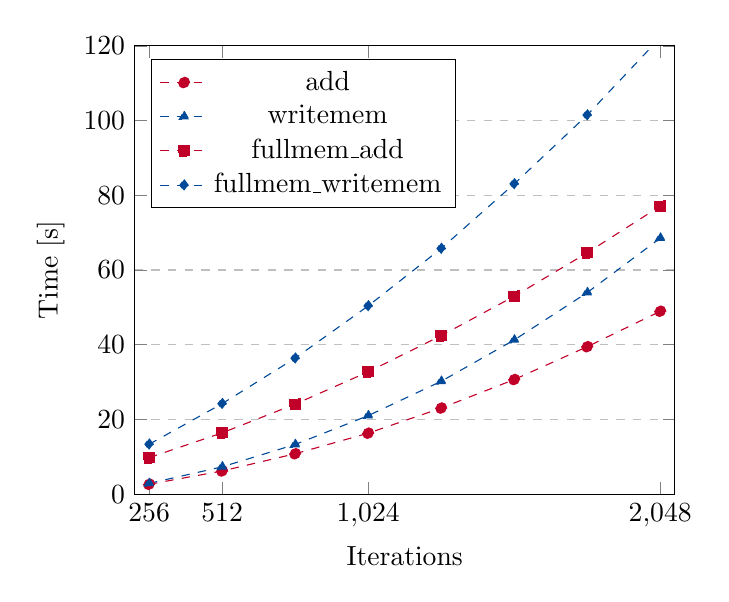
\begin{tikzpicture}
        \begin{axis}[
                xlabel={Iterations},
                ylabel={Time [s]},
                xmin=0206, xmax=2098,
                ymin=0, ymax=120,
                xtick={0256, 0512,1024,2048},
                ytick={0,20,40,60,80,100,120},
                legend pos=north west,
                ymajorgrids=true,
                grid style=dashed,
            ]

            \addplot[ color=UniRed, mark=*, dashed] coordinates { (0256, 2.635)
                    (0512, 6.195) (0768, 10.802) (1024, 16.306) (1280, 23.032) (1536,
                    30.669) (1792, 39.463) (2048, 48.944) };

            \addplot[ color= UniBlue, mark=triangle*, dashed] coordinates {
                    (0256,2.877) (0512,7.306) (0768,13.283) (1024,21.004) (1280,30.200)
                    (1536,41.262) (1792,53.940) (2048,68.521) };

            \addplot[ color= UniRed, mark=square*, dashed] coordinates {
                    (0256,9.759) (0512,16.402) (0768,24.093) (1024,32.732) (1280,42.410)
                    (1536,52.961) (1792,64.598) (2048,77.084) };

            \addplot[ color= UniBlue, mark=diamond*, dashed] coordinates { (0256,
                    13.344) (0512, 24.209) (0768, 36.388) (1024, 50.376) (1280, 65.746)
                    (1536, 83.036) (1792, 101.475) (2048, 122.189) }; \legend{add,
                writemem, fullmem\_add, fullmem\_writemem}

        \end{axis}
    \end{tikzpicture}

    \caption[Plotted iterations based benchmark
        times]{\tabref{tab:time_iter} plotted}
\end{figure}
\section{Results}
\begin{table}
    \centering
    \begin{tabular}{r|rr|rr|r}
        loops & \multicolumn{2}{c|}{base} & \multicolumn{2}{c|}{fullmem} & nopc                      \\
              & add                       & writemem                     & add    & writemem & add   \\ \hline
        0256  & 2.635                     & 2.877                        & 9.759  & 13.344   & 0.136 \\
        0512  & 6.195                     & 7.306                        & 16.402 & 24.209   & 0.268 \\
        0768  & 10.802                    & 13.283                       & 24.093 & 36.388   & 0.414 \\
        1024  & 16.306                    & 21.004                       & 32.732 & 50.376   & 0.569 \\
        1280  & 23.032                    & 30.200                       & 42.410 & 65.746   & 0.728 \\
        1536  & 30.669                    & 41.262                       & 52.961 & 83.036   & 0.898 \\
        1792  & 39.463                    & 53.940                       & 64.598 & 101.475  & 1.075 \\
        2048  & 48.944                    & 68.521                       & 77.084 & 122.189  & 1.276 \\
    \end{tabular}
    \caption{Times of iterations based benchmarks}\label{tab:time_iter}
\end{table}

\begin{table}
    \centering
    \begin{tabular}{r|rrrrr}
        bits of address space & 16     & 17            & 18     & 19     & 20     \\\hline
        add\_0256             & 2.635  & 2.632         & 2.626  & 2.626  & 2.624  \\
        add\_1024             & 16.306 & 16.464        & 16.511 & 16.452 & 16.460 \\

        writemem\_0256        & 2.877  & 2.88          & 2.890  & 2.889  & 2.890  \\
        writemem\_1024        & 21.004 & 21.131 21.215 & 21.181 & 21.163          \\

    \end{tabular}
    \caption{Times of extended address space benchmarks}\label{tab:time_extaddr}
\end{table}


\chapter{Conclusion}
I developed tools to transition from a state to a model and from a
witness of this model back to a state. Additionally, I implemented a
fuzzer for the states to verify the correct functioning of the model,
as well as a set of basic tests to benchmark its performance.
Finally, I presented and discussed the results of these benchmarks,
concluding that model checkers which appear superior in general are
worse at this specific task of mainly running iterations.


% If you want a list of your ToDos at the end of the document
% don't forget to remove before submission!
%% place it somewhere in the document
\chapter*{ToDo Counters}
\newcounter{ct}%
To Dos: \arabic{todos}; \hspace{1em}%
\setcounter{ct}{0}%
\whiledo {\value{ct} < \value{todos}}%
{%
	\stepcounter {ct}%
    \ref{todo \thect}%
	\ifnum\value{ct} = \value{todos}{}\else{, }\fi
}

Parts to extend: \arabic{extends}; \hspace{1em}%
\setcounter{ct}{0}%
\whiledo {\value{ct} < \value{extends}}%
{%
	\stepcounter {ct}%
	\ref{extend \thect}%
	\ifnum\value{ct} = \value{extends}{}\else{, }\fi
}

Draft parts: \arabic{drafts}; \hspace{1em}%
\setcounter{ct}{0}%
\whiledo {\value{ct} < \value{drafts}}%
{%
	\stepcounter {ct}%
	\ref{draft \thect}%
	\ifnum\value{ct} = \value{drafts}{}\else{, }\fi
}


\bibliographystyle{IEEEtran} \bibliography{bib/main,bib/additional}
% bibliography is not in the table of contents per default, add it manually
% enable the \renewcommand for german header
% \renewcommand{\bibname}{Literaturverzeichnis}
\addcontentsline{toc}{chapter}{Bibliography} \newpage
\thispagestyle{empty} \mbox{}

\todo{Add repo versions}

\end{document}
